\documentclass[journal, spanish]{IEEEtran}

% Paquetes necesarios
\usepackage[T1]{fontenc}
\usepackage[utf8]{inputenc}
\usepackage{babel}
\usepackage{cite}
\usepackage{graphicx}
\usepackage{float}


% Configuración de las cabeceras
\markboth{Estructuras De Datos}{Taller No. 1}


% Configuración de las secciones
\title{Taller No. 1}
\author{James Andres Cespedes Ibarra\thanks{} \\
\textit{Fundación Universitaria Konrad Lorenz} \\
}
\begin{document}

% Creación del título
\maketitle

% Creación del abstract
\begin{abstract}

Analizaremos fragmentos de código mediante notación Big-O con el fin de reforzar habilidades e interpretación de código y su complejidad.

\end{abstract}

% Resultados
\section{Resultados}

Después de realizado el ejercicio de la investigación podemos concluir que mediante el uso de la tecnología de análisis de datos bibliográficos podemos mejorar nuestra búsqueda en pro de realizar una mejor investigación y búsqueda en plataformas de registro bibliográfico

\subsection{Algoritmo No. 1}

\begin{figure}[H]
  \centering
  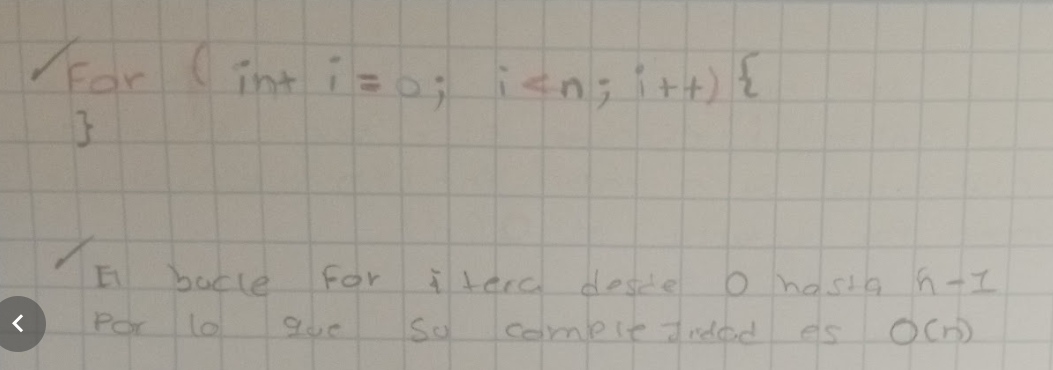
\includegraphics[width=0.5\textwidth]{images/Captura de pantalla 2023-09-13 025749.png}
  \caption{Análisis Escrito Del Algoritmo No. 1}
  \label{fig:nombre_de_tu_imagen}
\end{figure}

La complejidad temporal de este bucle es O(n), lo que significa que el tiempo de ejecución del bucle crecerá de manera lineal con el valor de n. Por lo tanto, si duplicas el valor de n, el tiempo de ejecución del bucle también se duplicará.

En resumen, este bucle for tiene una complejidad Big-O de O(n), lo que significa que su tiempo de ejecución es proporcional a la longitud del rango especificado por n.

\subsection{Algoritmo No. 2}

\begin{figure}[H]
  \centering
  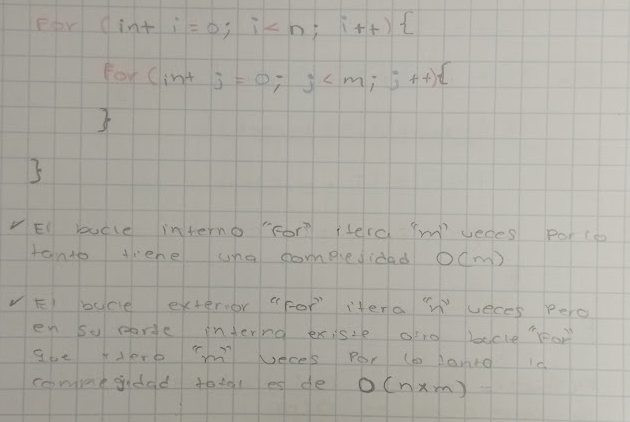
\includegraphics[width=0.5\textwidth]{images/Captura de pantalla 2023-09-13 030452.png}
  \caption{Análisis Escrito Del Algoritmo No. 2}
  \label{fig:nombre_de_tu_imagen}
\end{figure}

La complejidad temporal total de este código se puede expresar como O(n * m). Esto significa que el tiempo de ejecución de los bucles es proporcional al producto de n y m. Si tanto n como m son grandes, el tiempo de ejecución será mayor, y si son pequeños, el tiempo de ejecución será menor.

En resumen, este código tiene una complejidad Big-O de O(n * m) debido a los bucles anidados, lo que significa que su tiempo de ejecución es proporcional al producto de n y m.

\subsection{Algoritmo No. 3}

\begin{figure}[H]
  \centering
  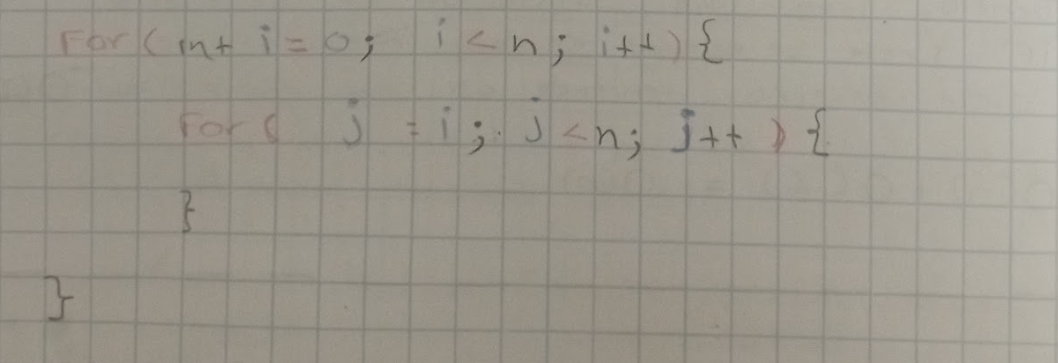
\includegraphics[width=0.5\textwidth]{images/Captura de pantalla 2023-09-13 030912.png}
  \caption{Análisis Escrito Del Algoritmo No. 3 - 1}
  \label{fig:nombre_de_tu_imagen}
\end{figure}

\begin{figure}[H]
  \centering
  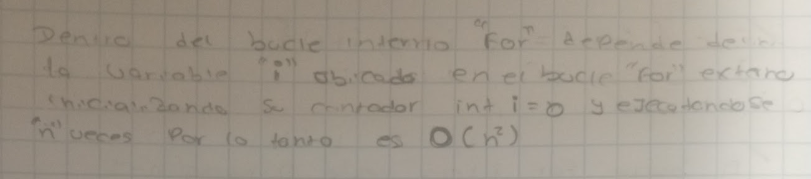
\includegraphics[width=0.5\textwidth]{images/Captura de pantalla 2023-09-13 030943.png}
  \caption{Análisis Escrito Del Algoritmo No. 3 - 2}
  \label{fig:nombre_de_tu_imagen}
\end{figure}

Este código tiene una complejidad Big-O de O$(n^2)$ debido a los bucles anidados, lo que significa que su tiempo de ejecución crece cuadráticamente con el valor de n.

\subsection{Algoritmo No. 4}

\begin{figure}[H]
  \centering
  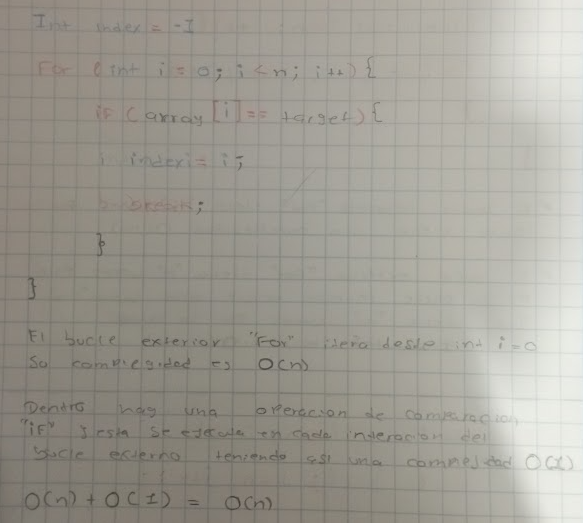
\includegraphics[width=0.5\textwidth]{images/Captura de pantalla 2023-09-13 032834.png}
  \caption{Análisis Escrito Del Algoritmo No. 4}
  \label{fig:nombre_de_tu_imagen}
\end{figure}

La complejidad temporal total de este código se puede expresar si el elemento target no está presente en el arreglo, el bucle for se ejecutará n veces antes de terminar sin haber encontrado el elemento. En este caso, la complejidad temporal es O(n).

\subsection{Algoritmo No. 5}

\begin{figure}[H]
  \centering
  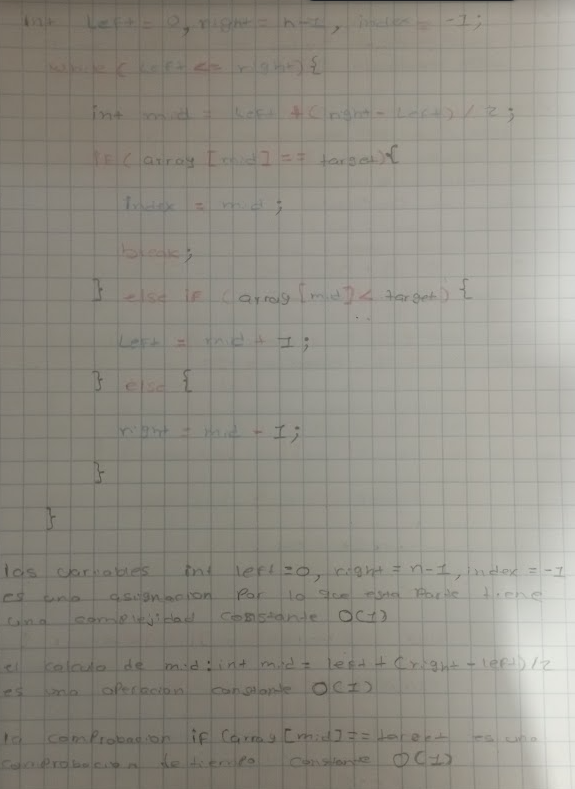
\includegraphics[width=0.5\textwidth]{images/Captura de pantalla 2023-09-13 033301.png}
  \caption{Análisis Escrito Del Algoritmo No. 5 - 1}
  \label{fig:nombre_de_tu_imagen}
\end{figure}

\begin{figure}[H]
  \centering
  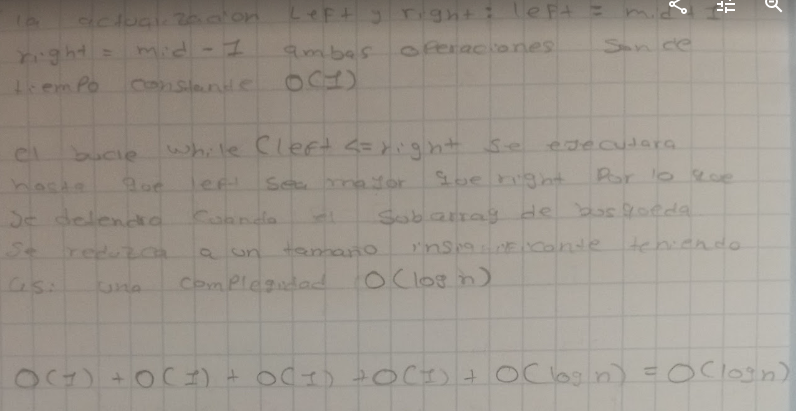
\includegraphics[width=0.5\textwidth]{images/Captura de pantalla 2023-09-13 033555.png}
  \caption{Análisis Escrito Del Algoritmo No. 5 - 2}
  \label{fig:nombre_de_tu_imagen}
\end{figure}

La complejidad temporal de este código de búsqueda binaria es O(log n), donde n es la longitud del arreglo. Esto significa que el tiempo de ejecución del algoritmo crece de manera logarítmica con el tamaño del arreglo.

\subsection{Algoritmo No. 6}

\begin{figure}[H]
  \centering
  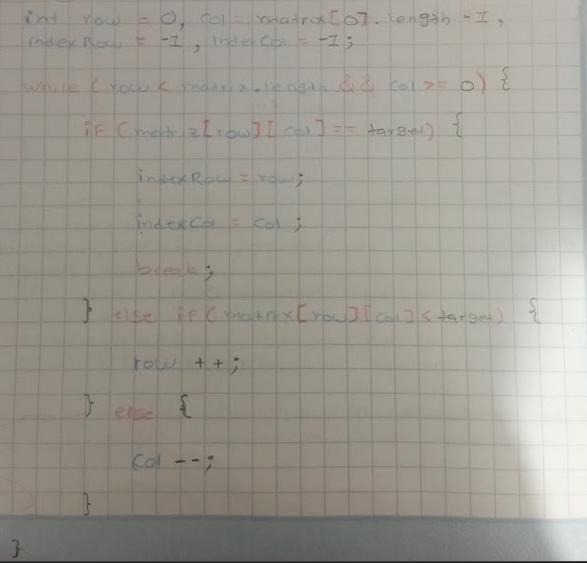
\includegraphics[width=0.5\textwidth]{images/Captura de pantalla 2023-09-13 033809.png}
  \caption{Análisis Escrito Del Algoritmo No. 6 - 1}
  \label{fig:nombre_de_tu_imagen}
\end{figure}

\begin{figure}[H]
  \centering
  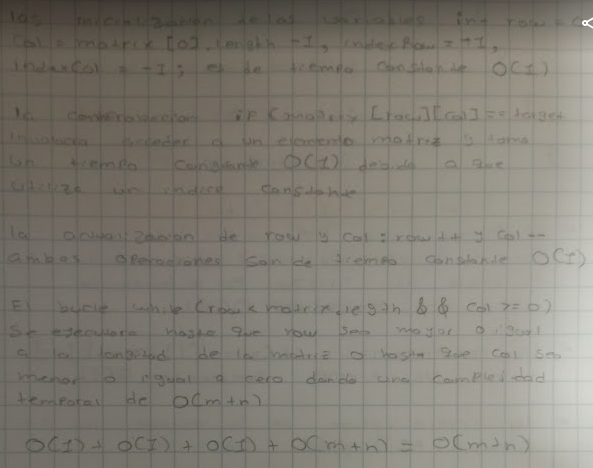
\includegraphics[width=0.5\textwidth]{images/Captura de pantalla 2023-09-13 033825.png}
  \caption{Análisis Escrito Del Algoritmo No. 6 - 2}
  \label{fig:nombre_de_tu_imagen}
\end{figure}

La complejidad temporal de este código de búsqueda en una matriz ordenada es Big-O de O(m + n), donde m es el número de filas de la matriz y n es el número de columnas de la matriz.

Esto significa que el tiempo de ejecución del algoritmo crece linealmente con el número de filas y columnas de la matriz.

\subsection{Algoritmo No. 7}

\begin{figure}[H]
  \centering
  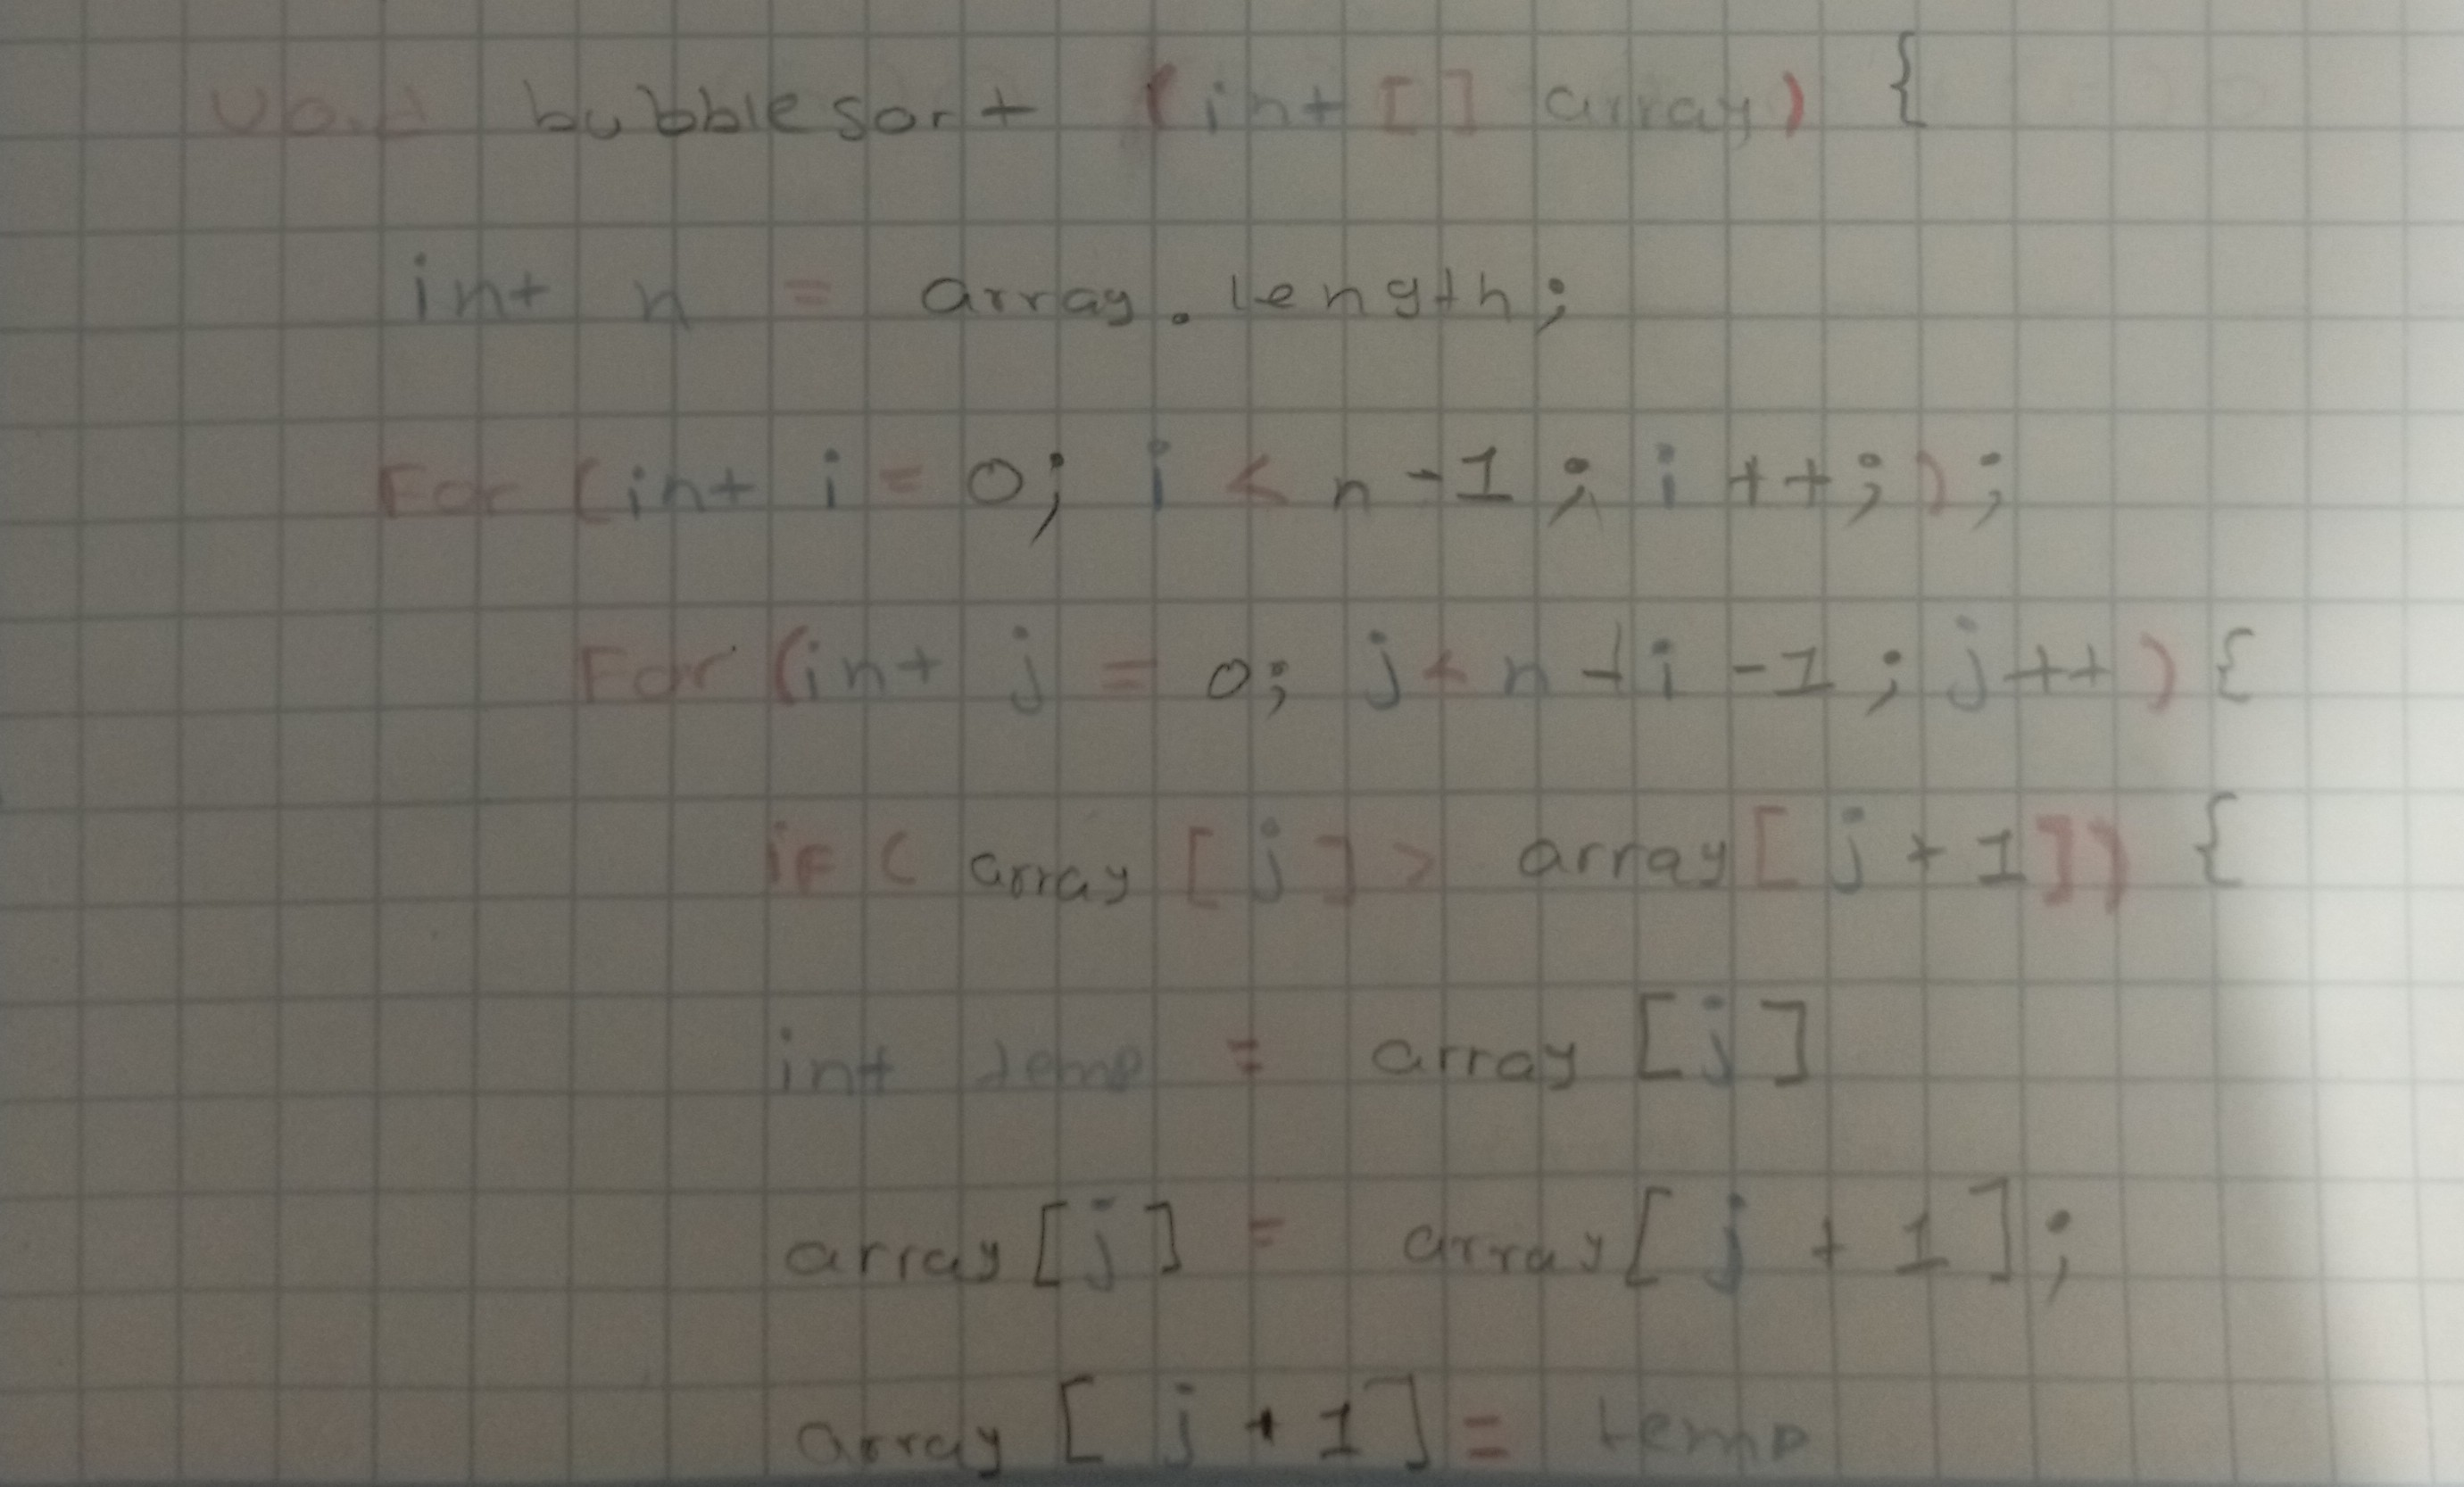
\includegraphics[width=0.5\textwidth]{images/IMG_20230913_023442~2.jpg}
  \caption{Análisis Escrito Del Algoritmo No. 7 - 1}
  \label{fig:nombre_de_tu_imagen}
\end{figure}

\begin{figure}[H]
  \centering
  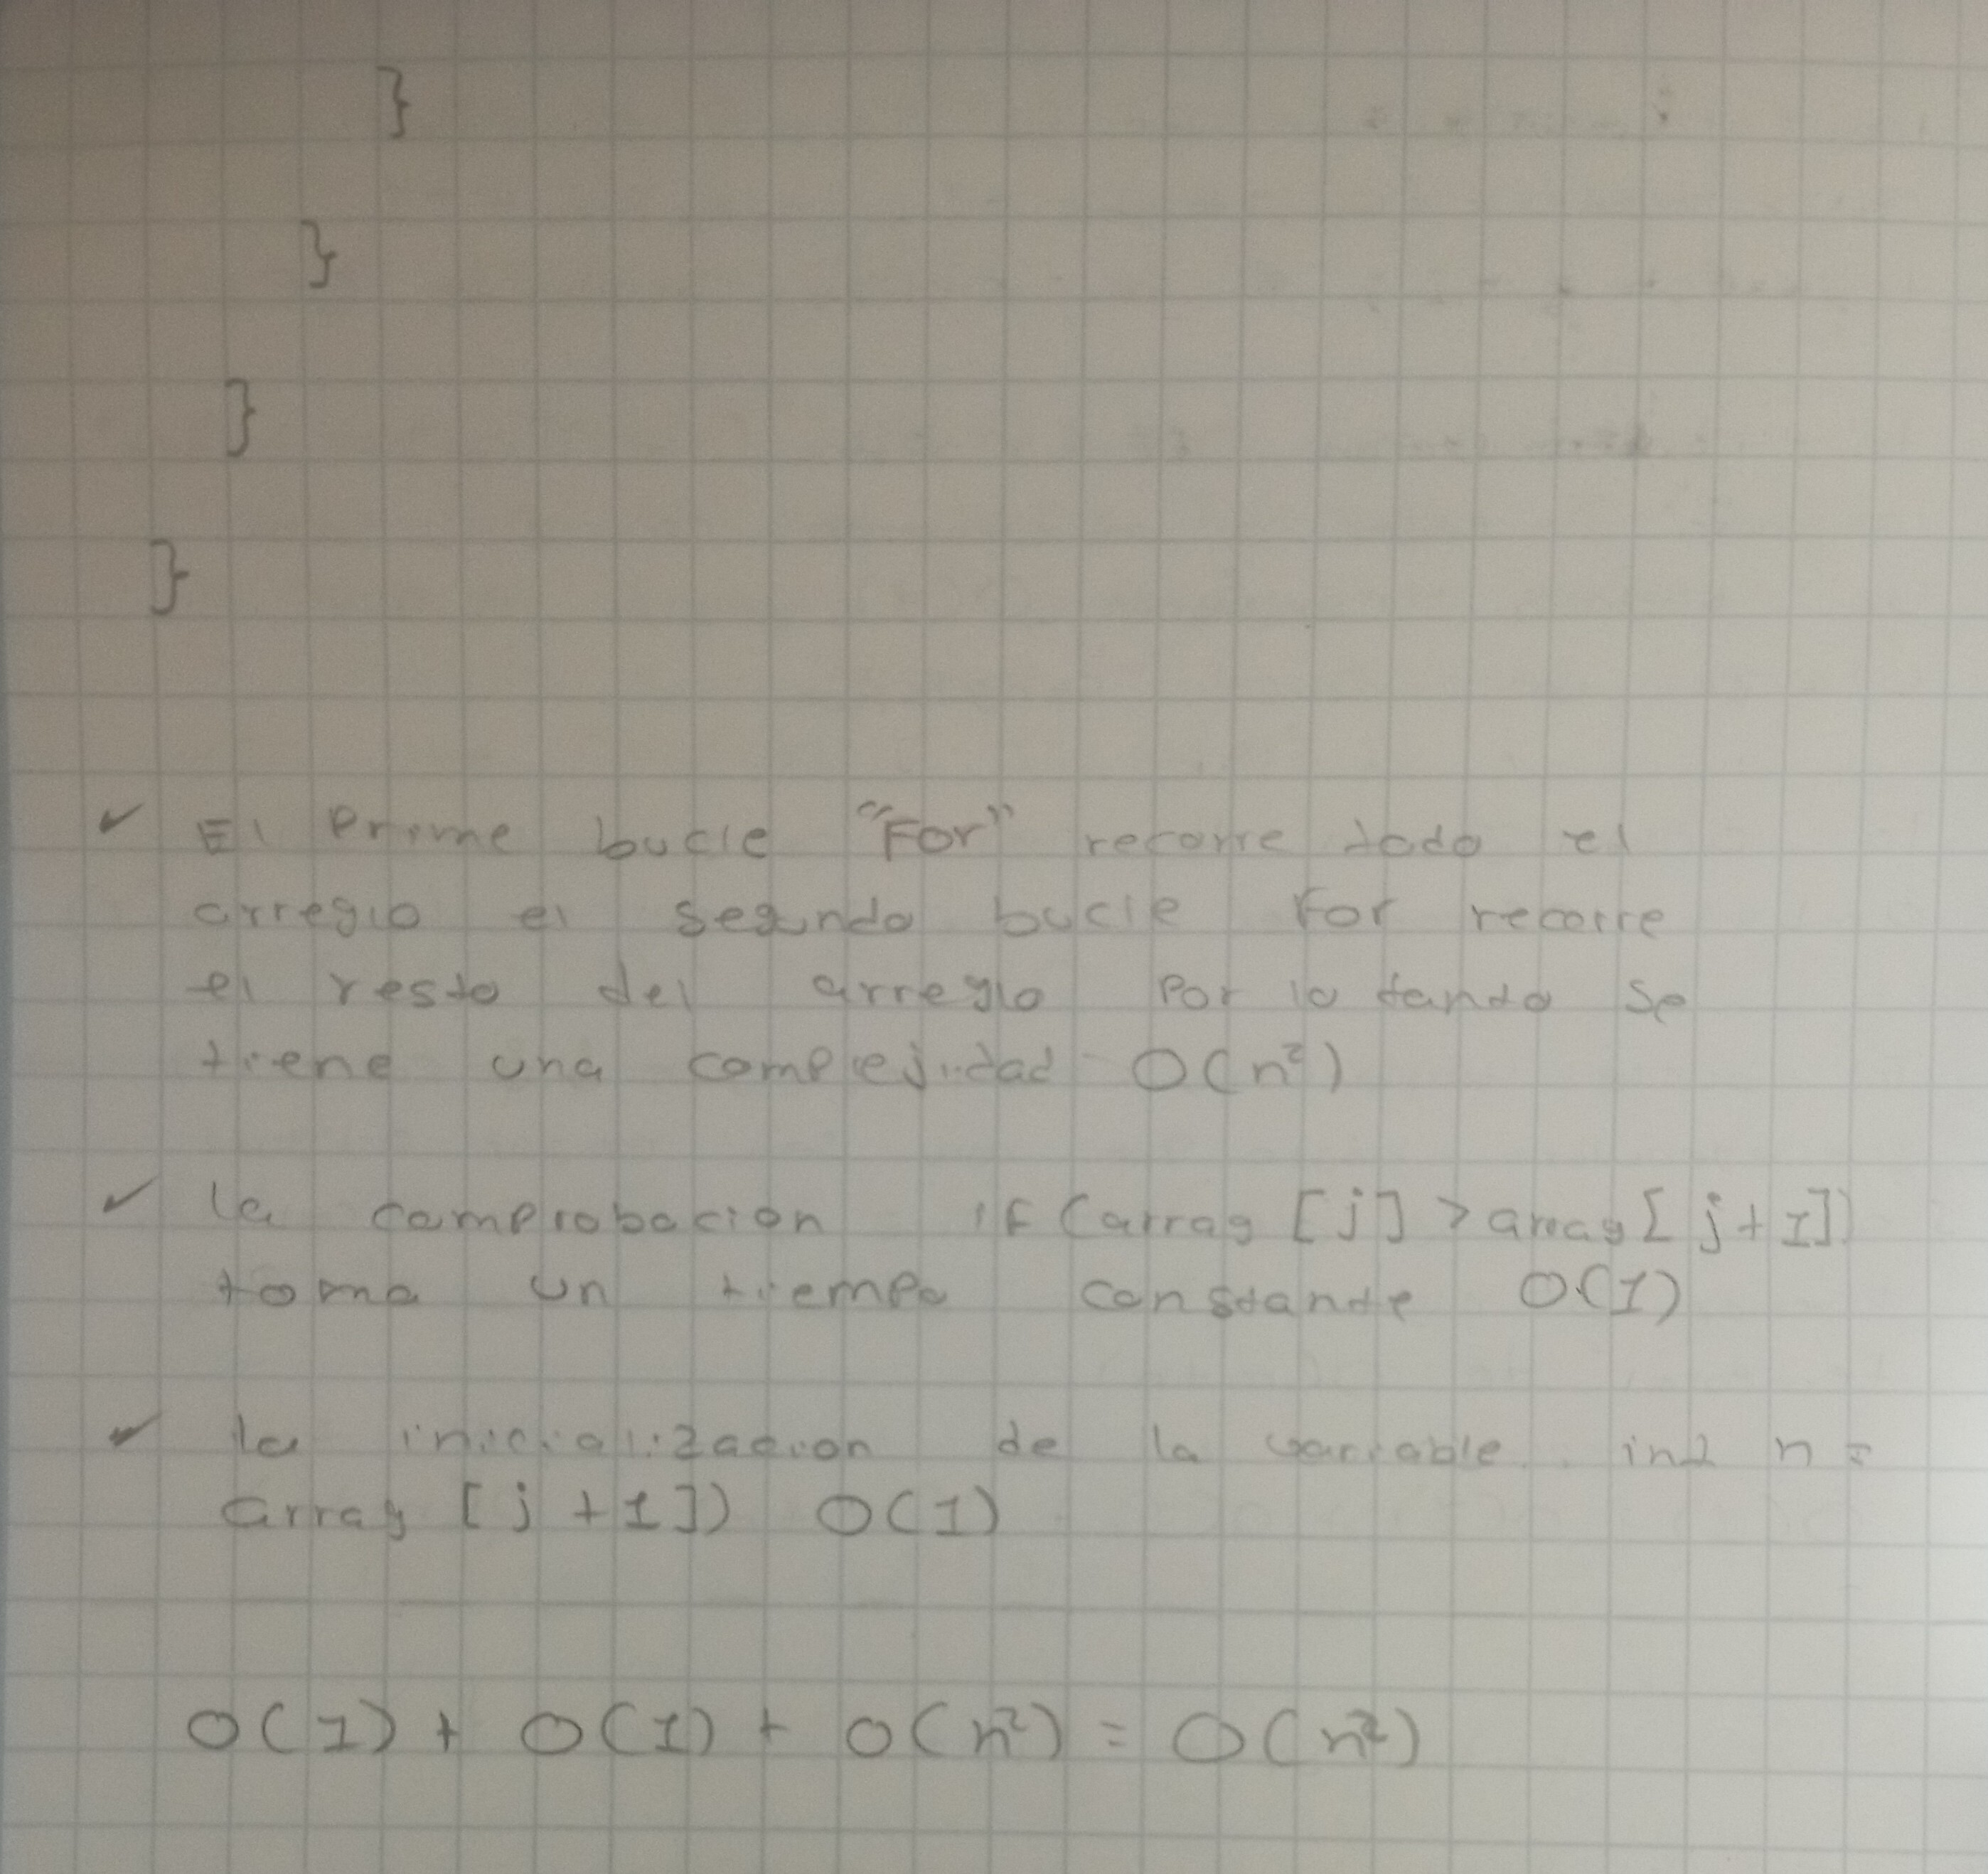
\includegraphics[width=0.5\textwidth]{images/IMG_20230913_023451~2.jpg}
  \caption{Análisis Escrito Del Algoritmo No. 7 - 2}
  \label{fig:nombre_de_tu_imagen}
\end{figure}

La complejidad temporal de este algoritmo de ordenación por burbuja tiene dos bucles anidados, lo que significa que se realizarán "n-1" comparaciones e intercambios en la primera iteración, "n-2" en la segunda, y así sucesivamente hasta una comparación e intercambio en la última iteración. Esto da como resultado una complejidad temporal Big-O de O$(n^2)$, donde "n" es la longitud del array.

\subsection{Algoritmo No. 8}

\begin{figure}[H]
  \centering
  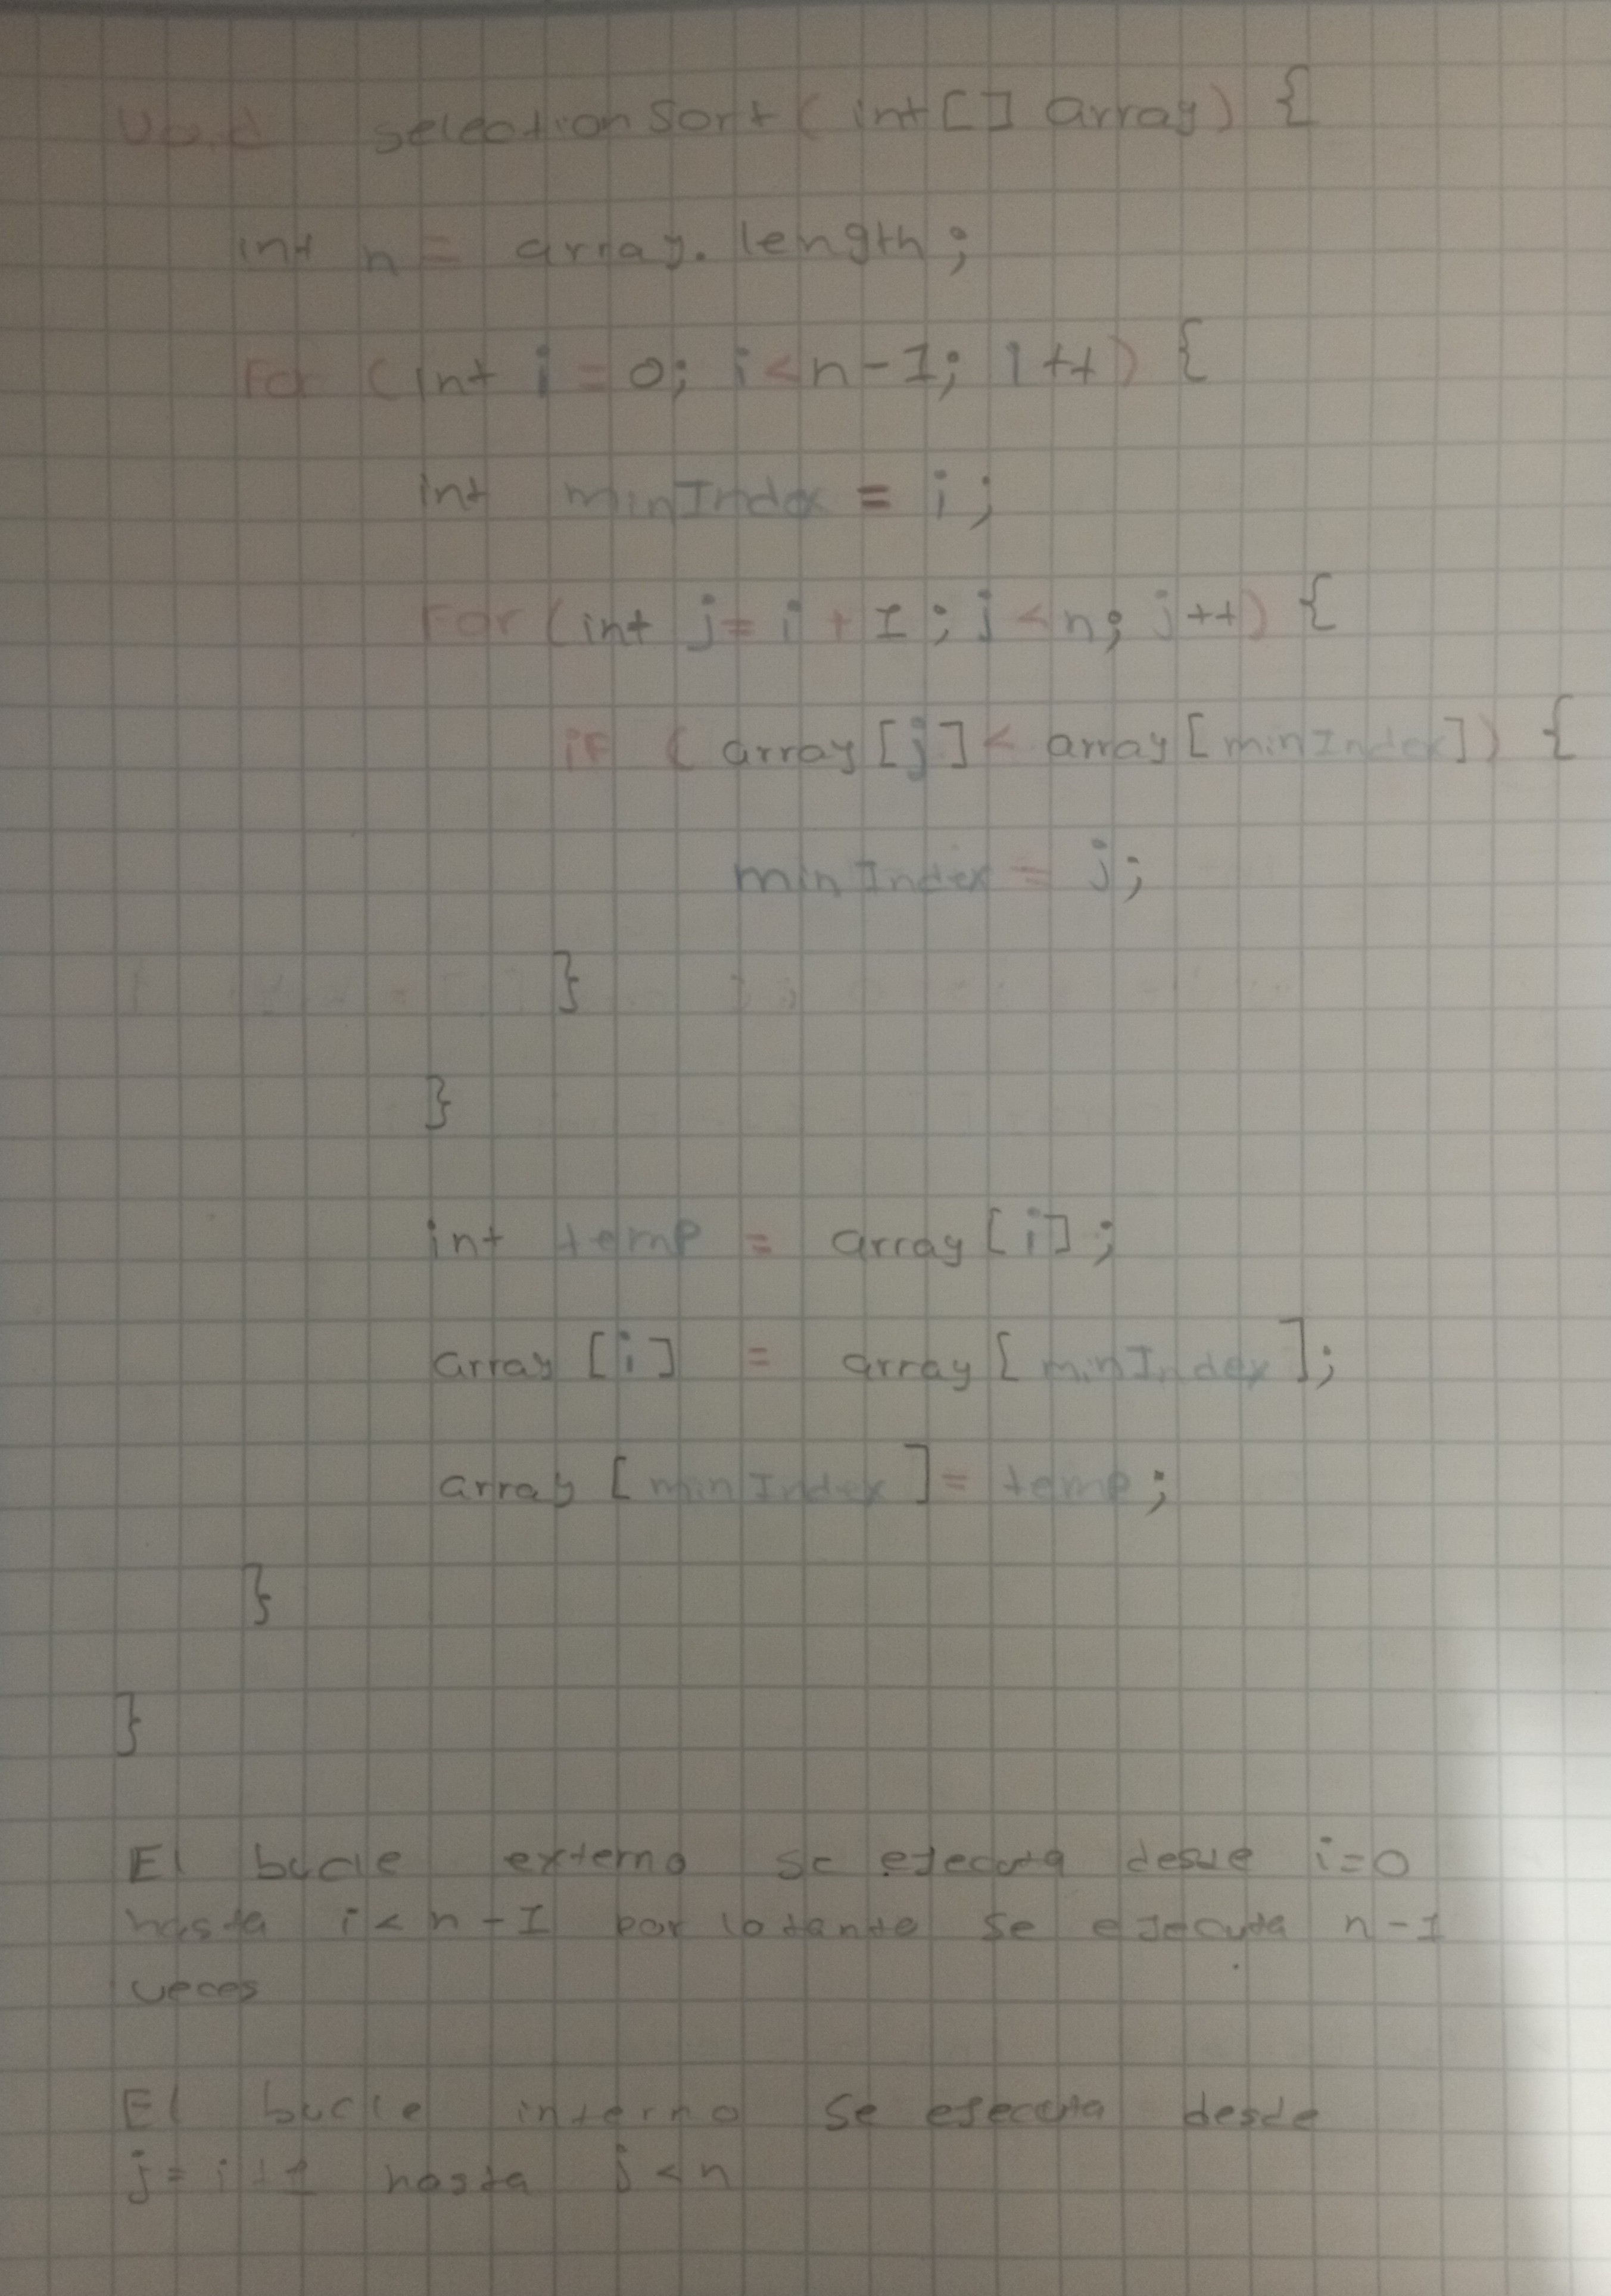
\includegraphics[width=0.5\textwidth]{images/IMG_20230913_023459~2.jpg}
  \caption{Análisis Escrito Del Algoritmo No. 8 - 1}
  \label{fig:nombre_de_tu_imagen}
\end{figure}

\begin{figure}[H]
  \centering
  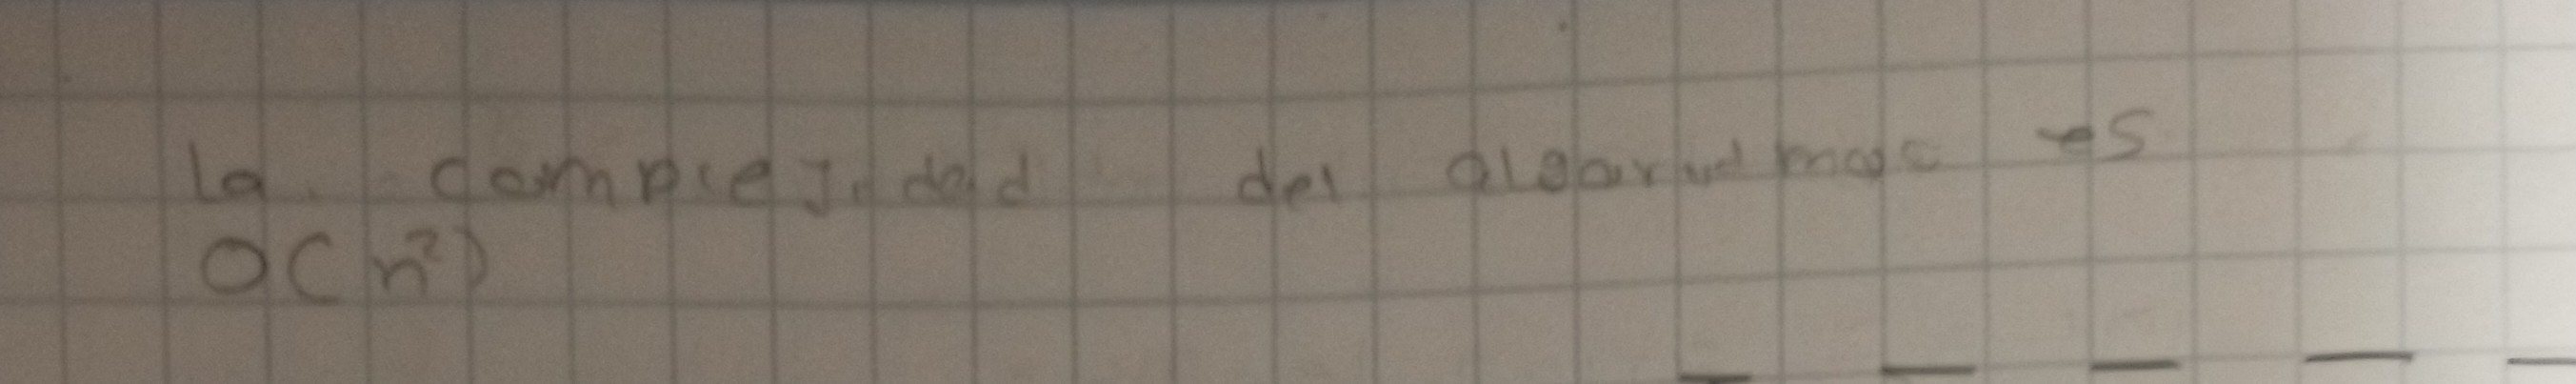
\includegraphics[width=0.5\textwidth]{images/IMG_20230913_023543~2.jpg}
  \caption{Análisis Escrito Del Algoritmo No. 8 - 2}
  \label{fig:nombre_de_tu_imagen}
\end{figure}

La complejidad temporal de este algoritmo de ordenación por selección tiene dos bucles anidados y realiza intercambios de elementos en función de encontrar el elemento mínimo en la porción no ordenada del array en cada iteración del bucle externo. La complejidad temporal de Selection Sort es Big-O de O$(n^2)$ donde "n" es la longitud del array.

\subsection{Algoritmo No. 9}

\begin{figure}[H]
  \centering
  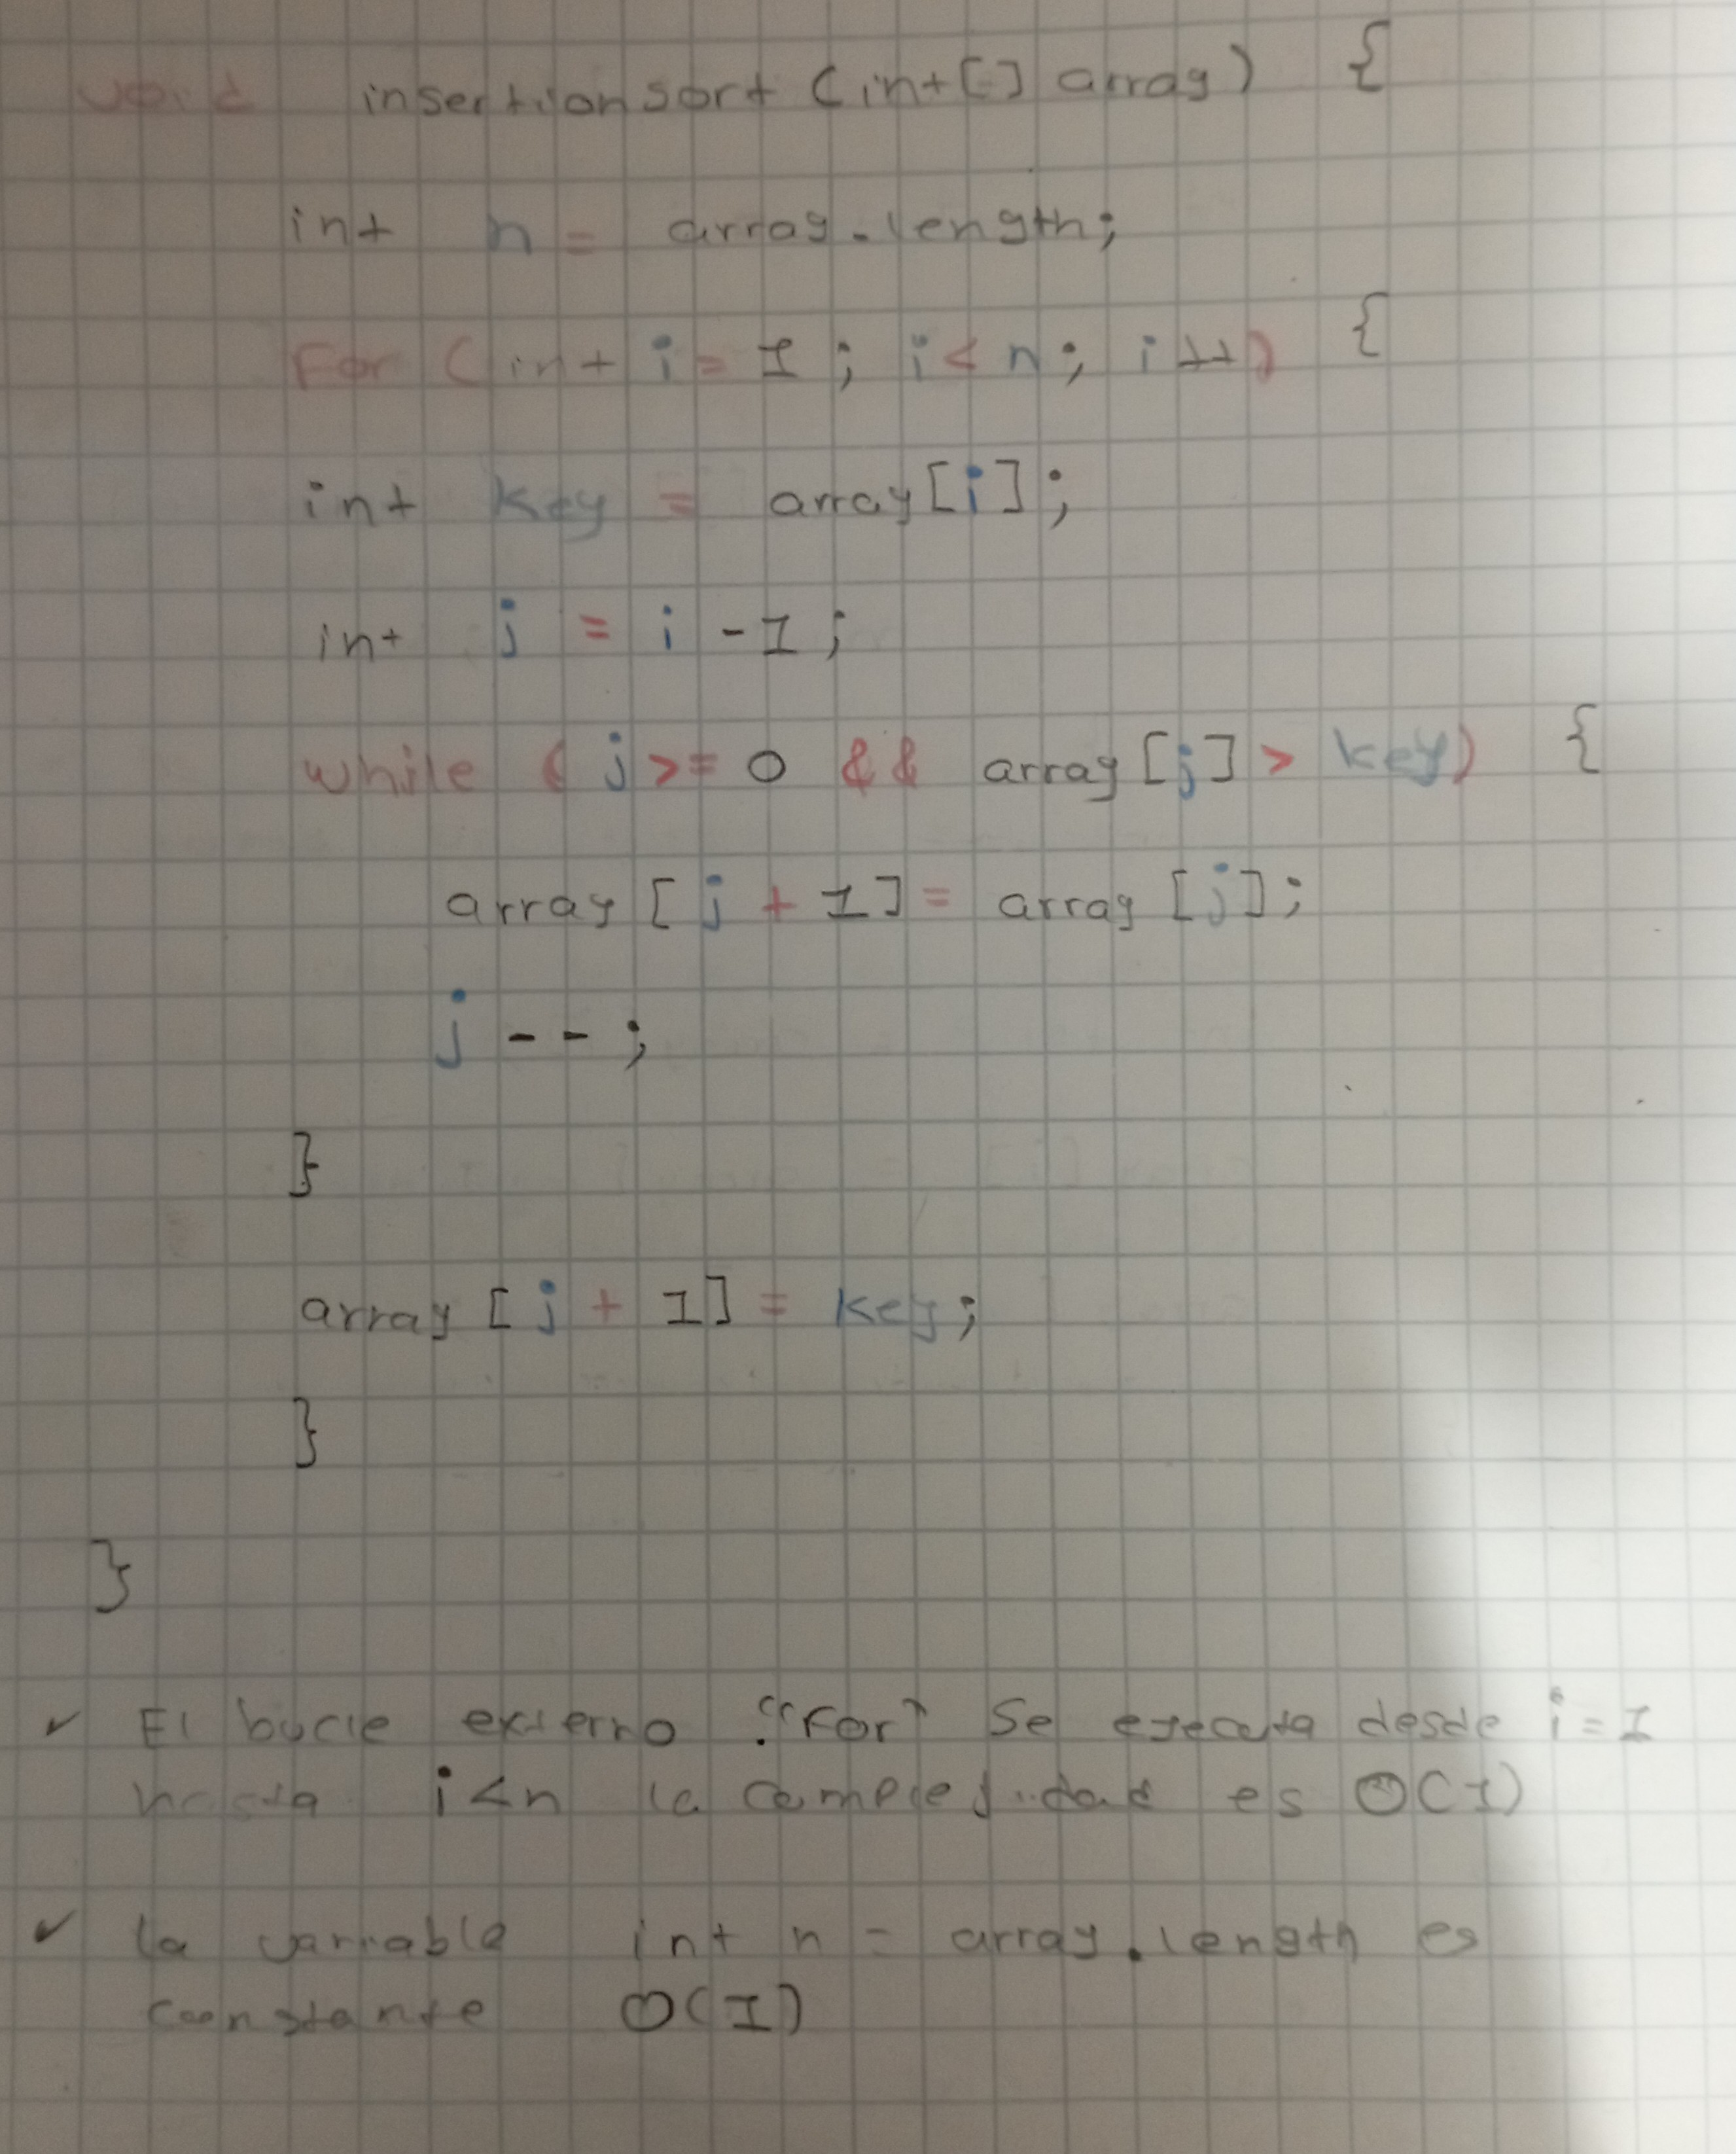
\includegraphics[width=0.5\textwidth]{images/IMG_20230913_023543~3.jpg}
  \caption{Análisis Escrito Del Algoritmo No. 9 - 1}
  \label{fig:nombre_de_tu_imagen}
\end{figure}

\begin{figure}[H]
  \centering
  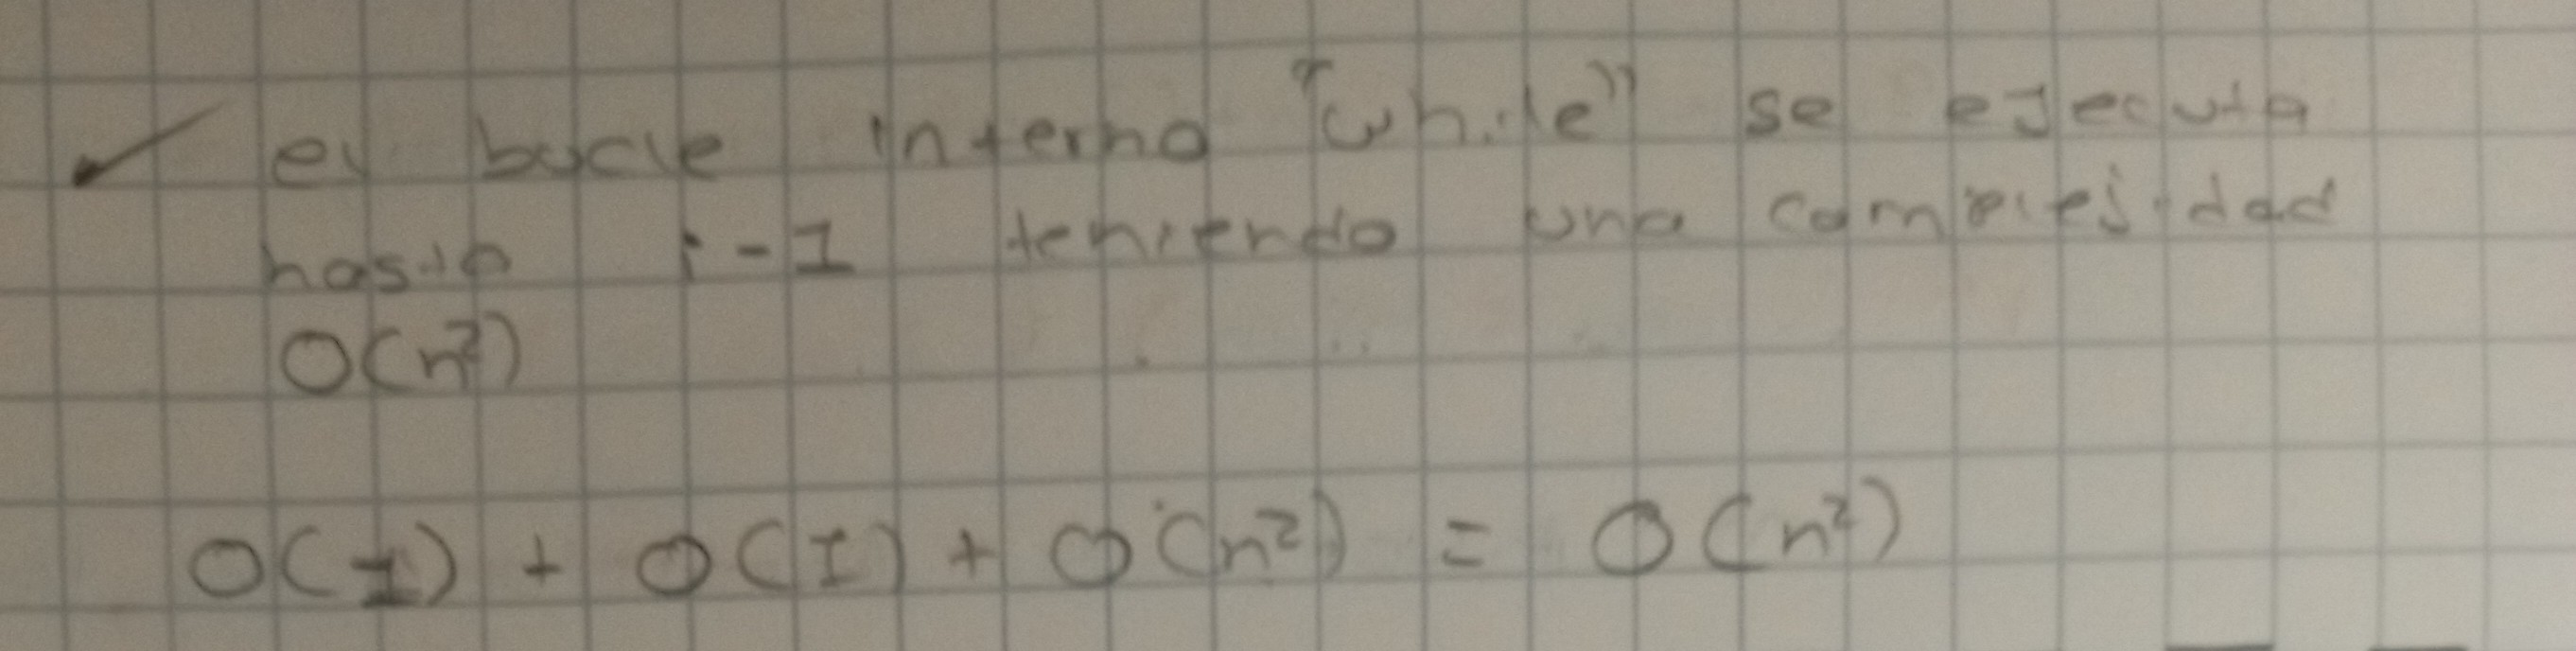
\includegraphics[width=0.5\textwidth]{images/IMG_20230913_023549~2.jpg}
  \caption{Análisis Escrito Del Algoritmo No. 9 - 2}
  \label{fig:nombre_de_tu_imagen}
\end{figure}

La complejidad temporal de este algoritmo de ordenación por inserción tiene un bucle externo que recorre el array una vez y un bucle interno que realiza comparaciones e intercambios mientras se ajusta el elemento en su posición correcta en la parte ordenada del array. La complejidad temporal de Insertion Sort es Big-O de O$(n^2)$, donde "n" es la longitud del array.

\subsection{Algoritmo No. 10}

\begin{figure}[H]
  \centering
  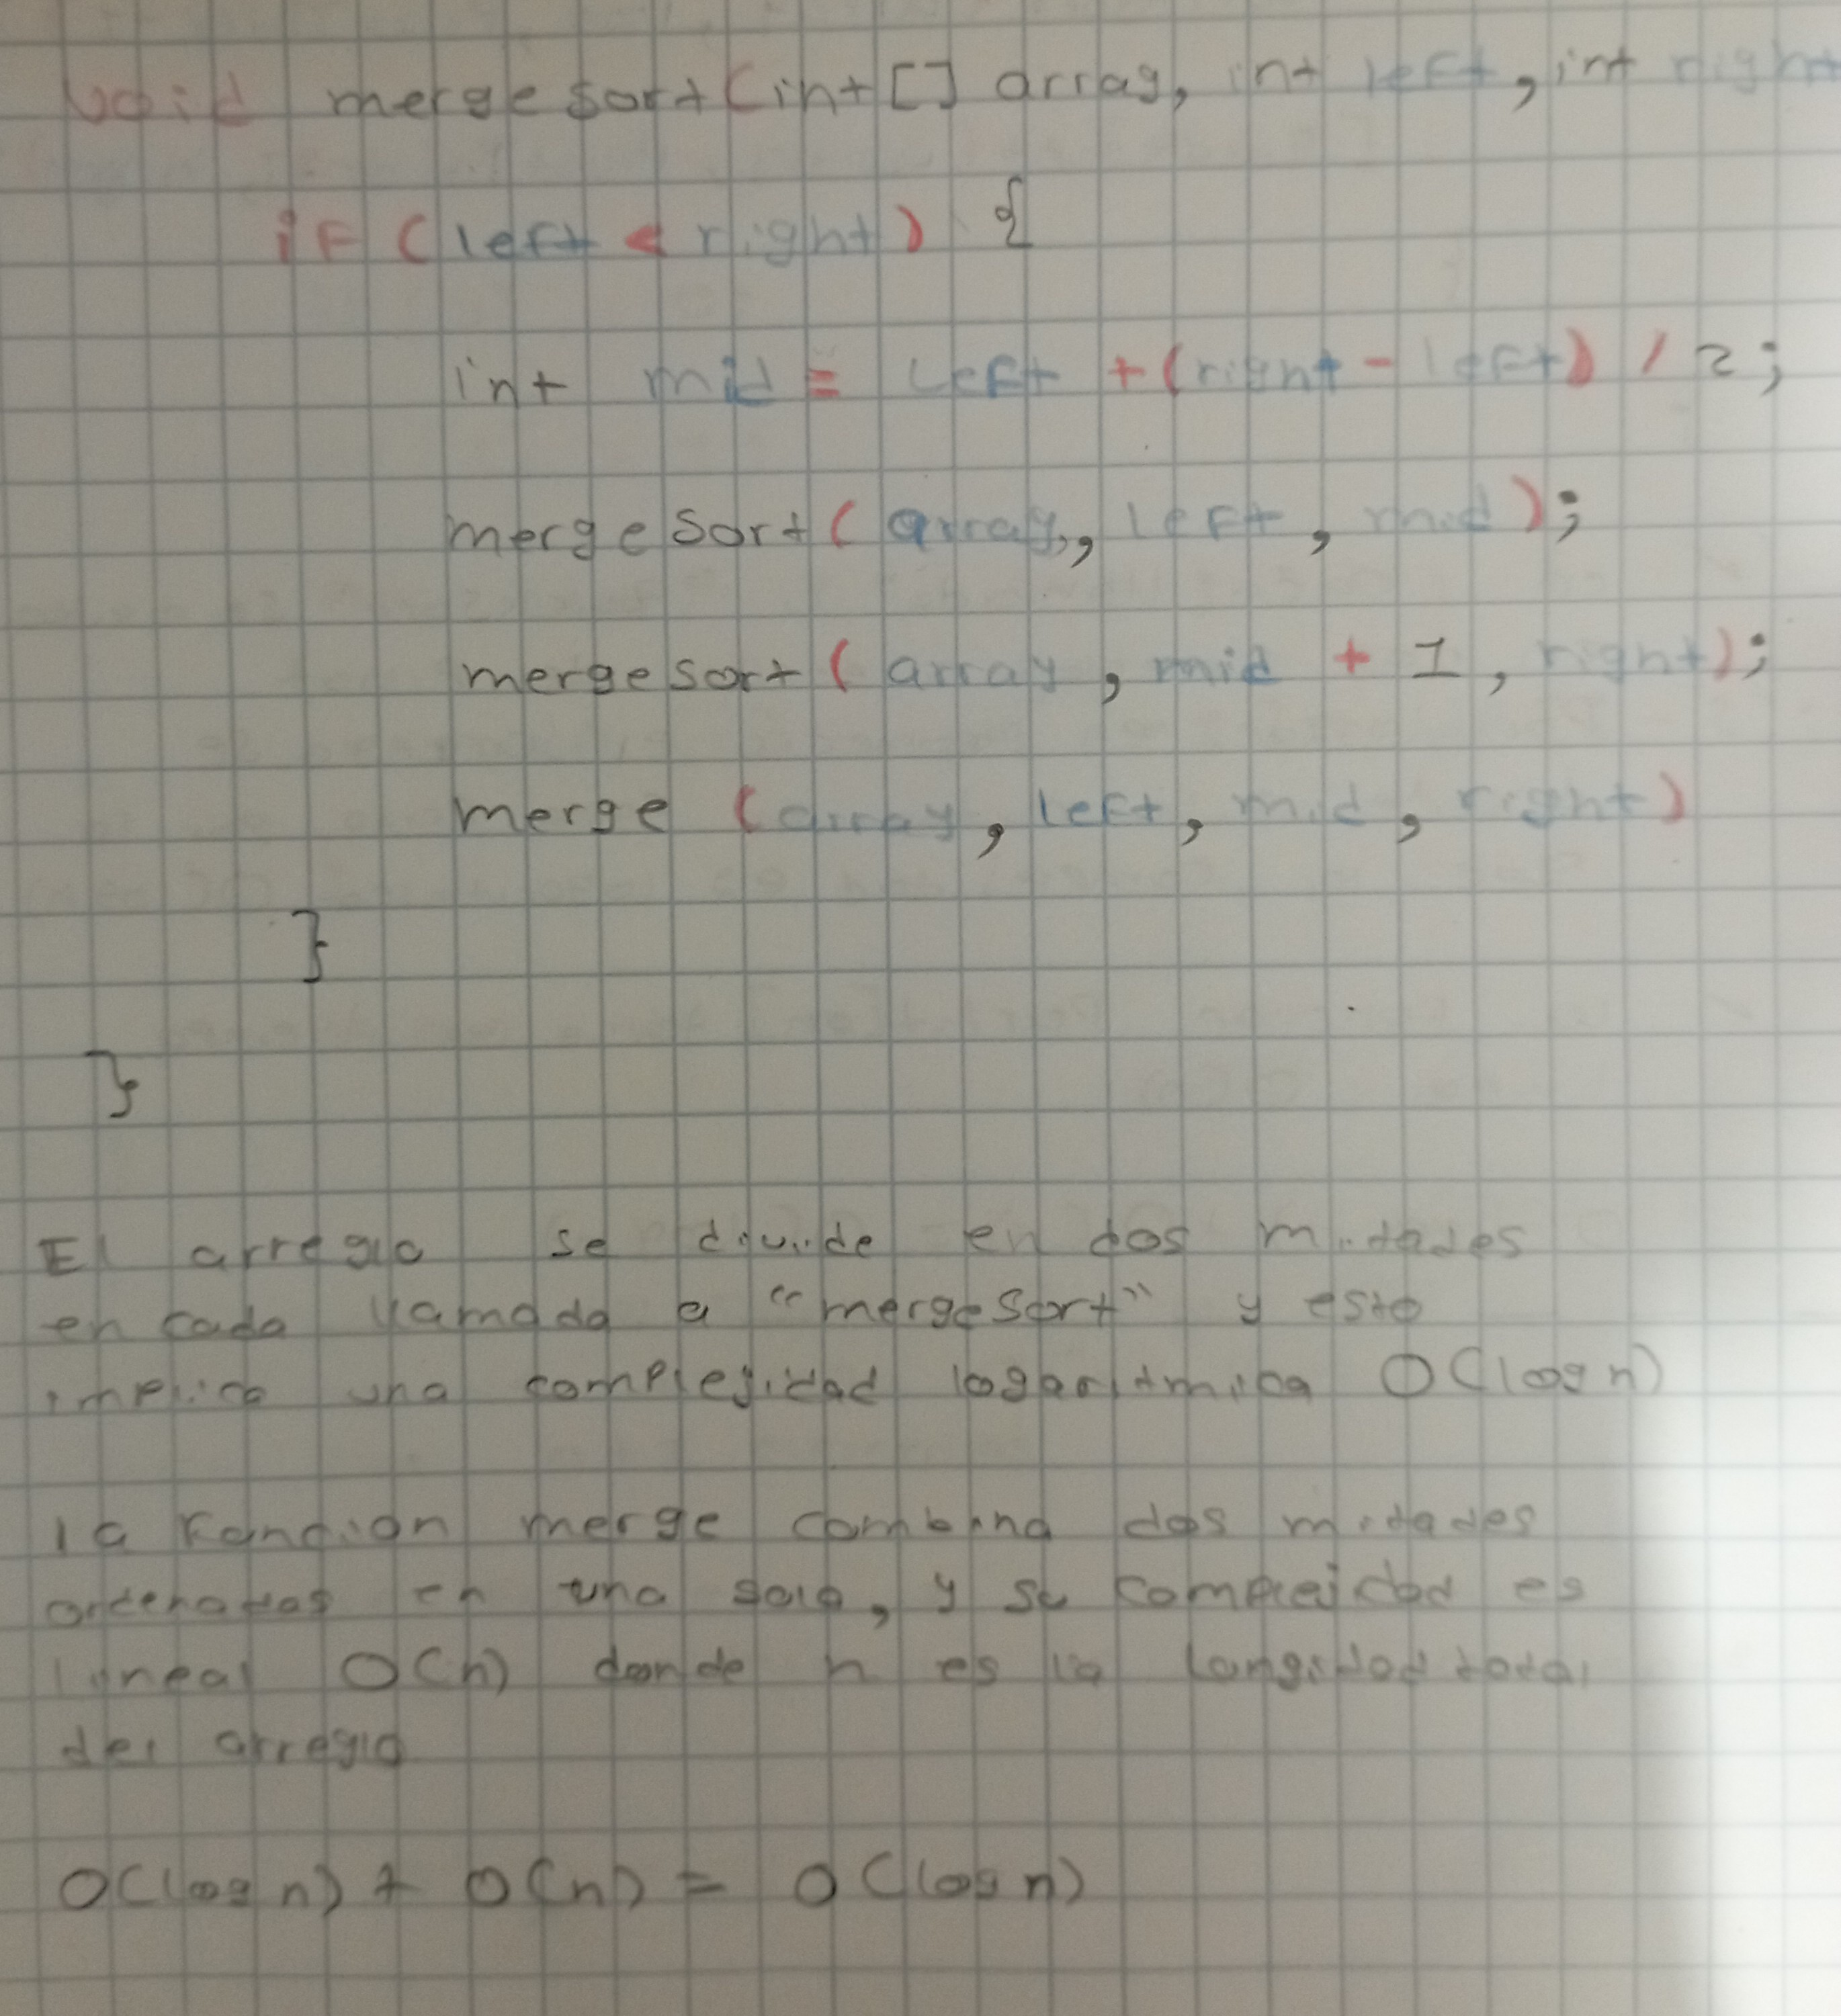
\includegraphics[width=0.5\textwidth]{images/IMG_20230913_023549~3.jpg}
  \caption{Análisis Escrito Del Algoritmo No. 10}
  \label{fig:nombre_de_tu_imagen}
\end{figure}

La complegidad temporal de este algoritmo de ordenación eficiente con una complejidad temporal Big-O O(n log n)

\subsection{Algoritmo No. 11}

\begin{figure}[H]
  \centering
  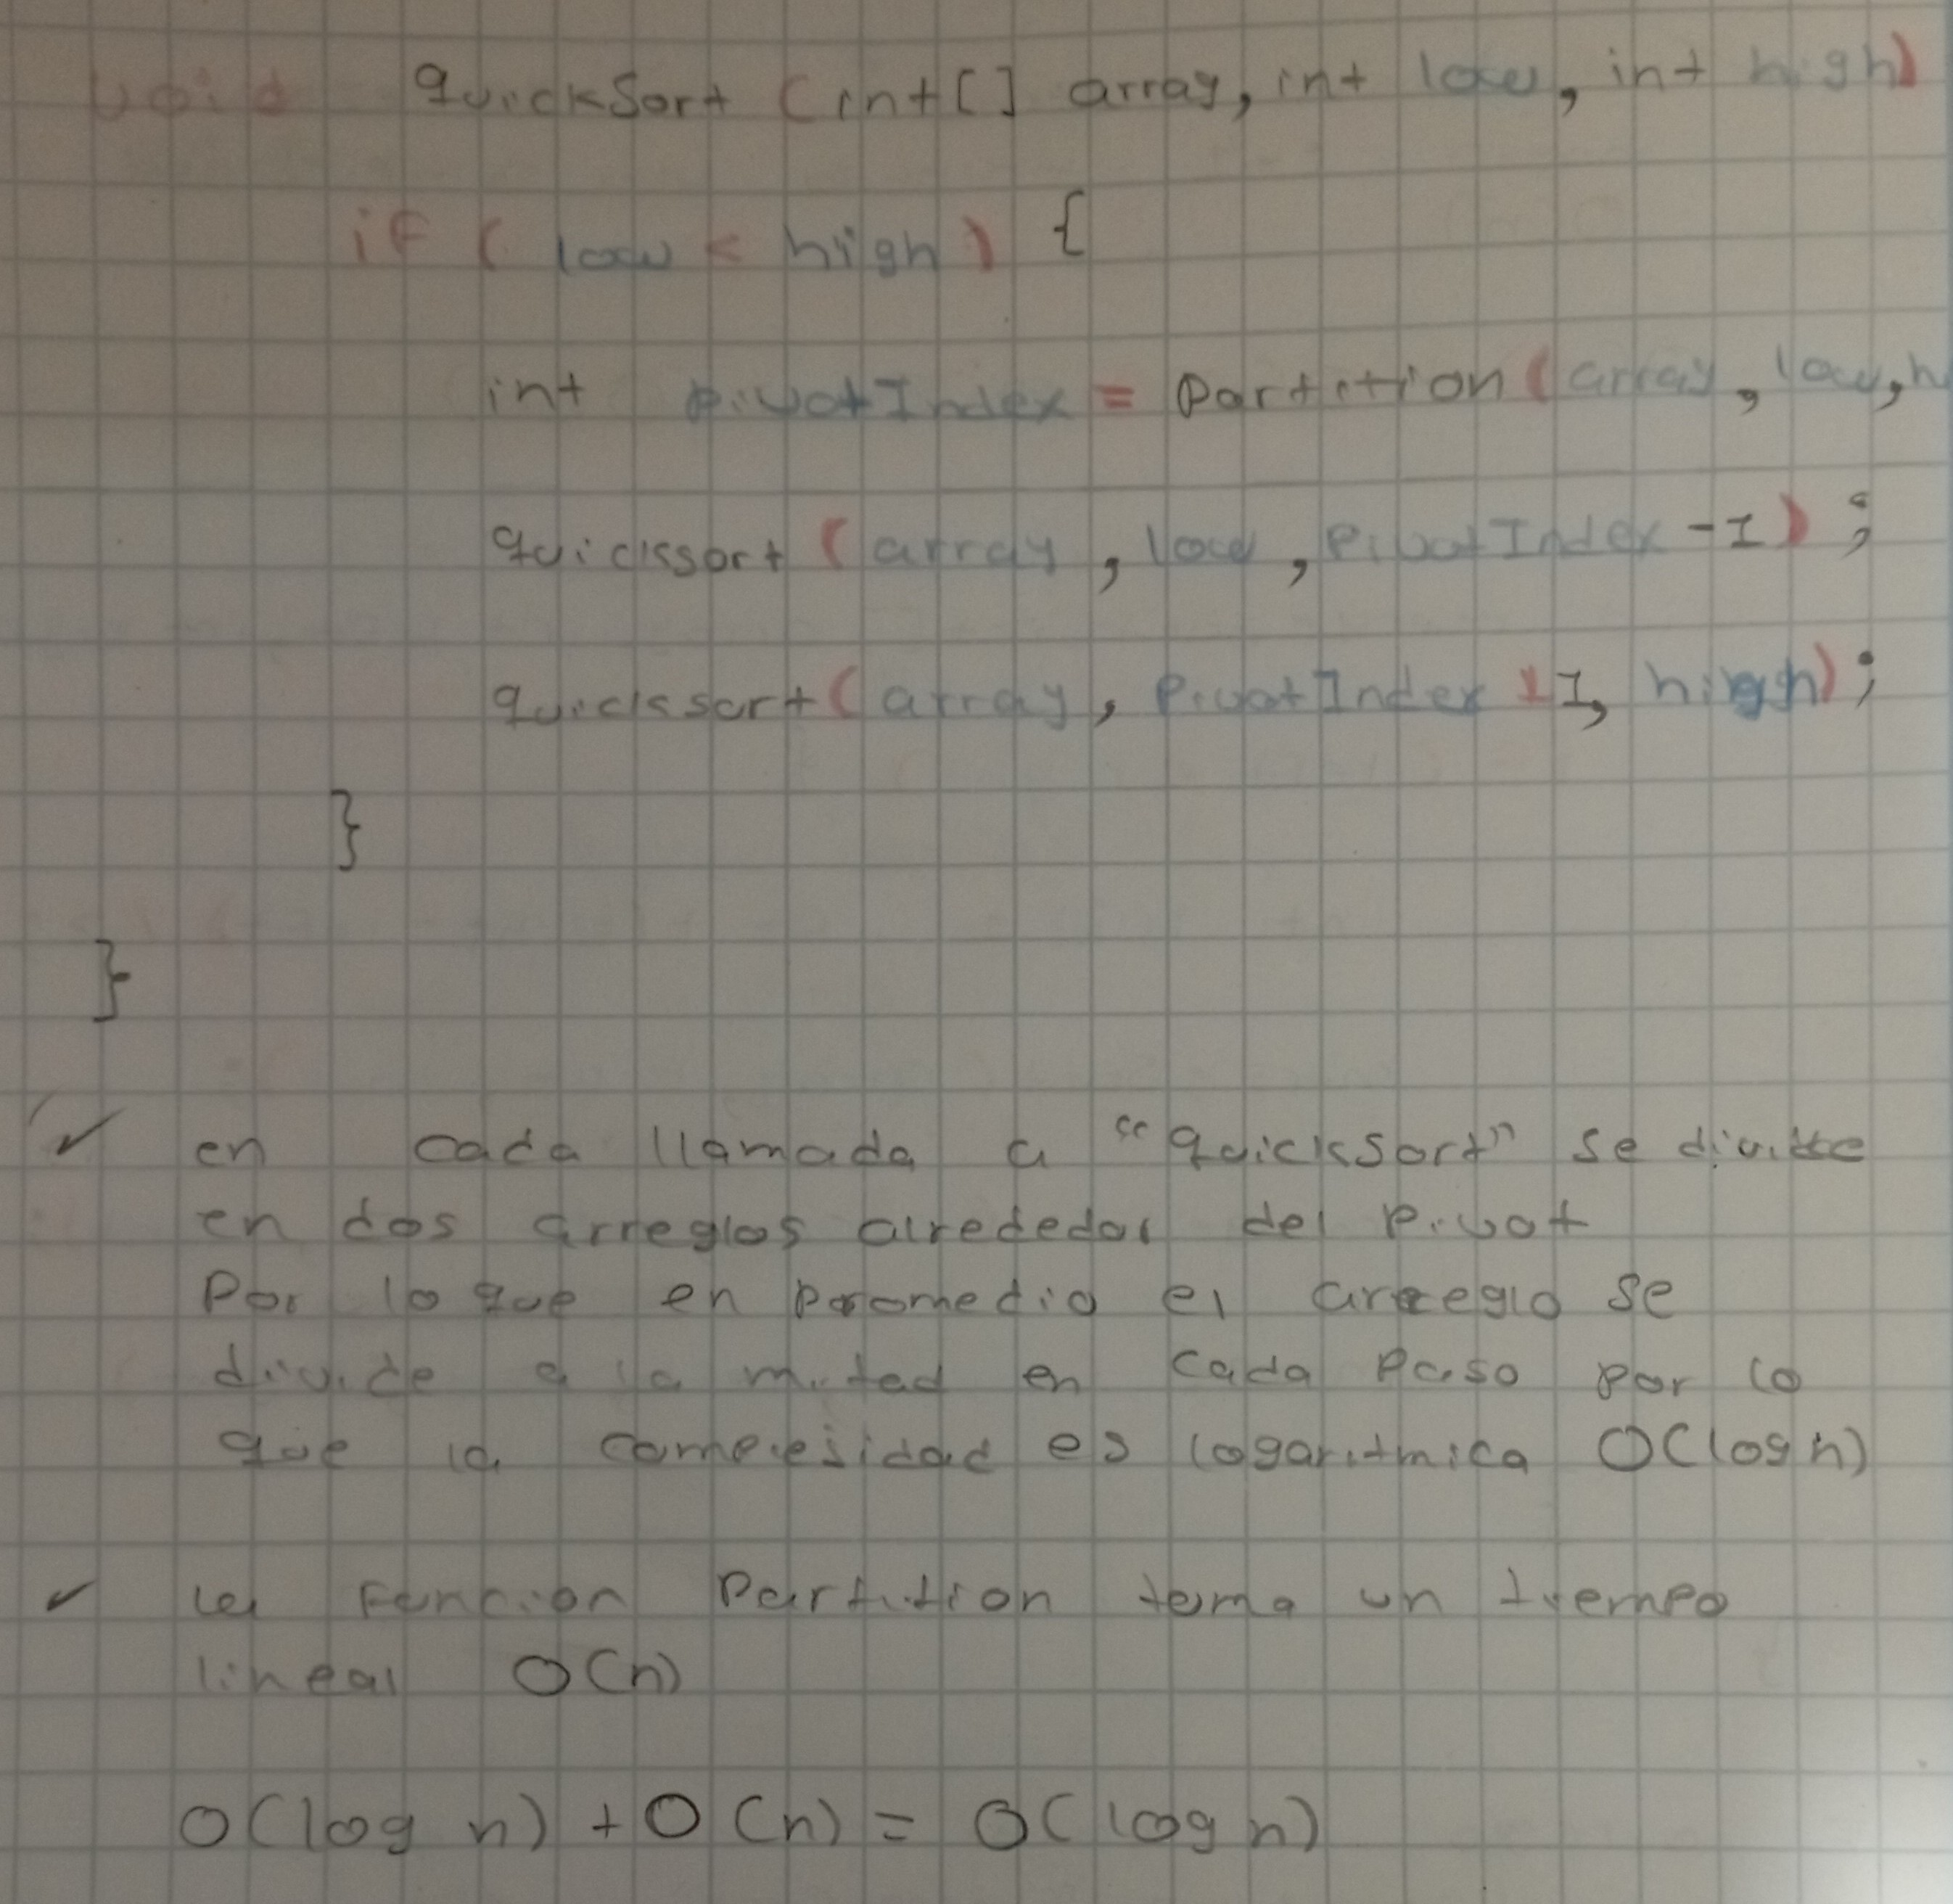
\includegraphics[width=0.5\textwidth]{images/IMG_20230913_023605~2.jpg}
  \caption{Análisis Escrito Del Algoritmo No. 11}
  \label{fig:nombre_de_tu_imagen}
\end{figure}

La complegidad temporal de este algoritmo de ordenación es de Big-O O$(n^2)$.

\subsection{Algoritmo No. 12}

\begin{figure}[H]
  \centering
  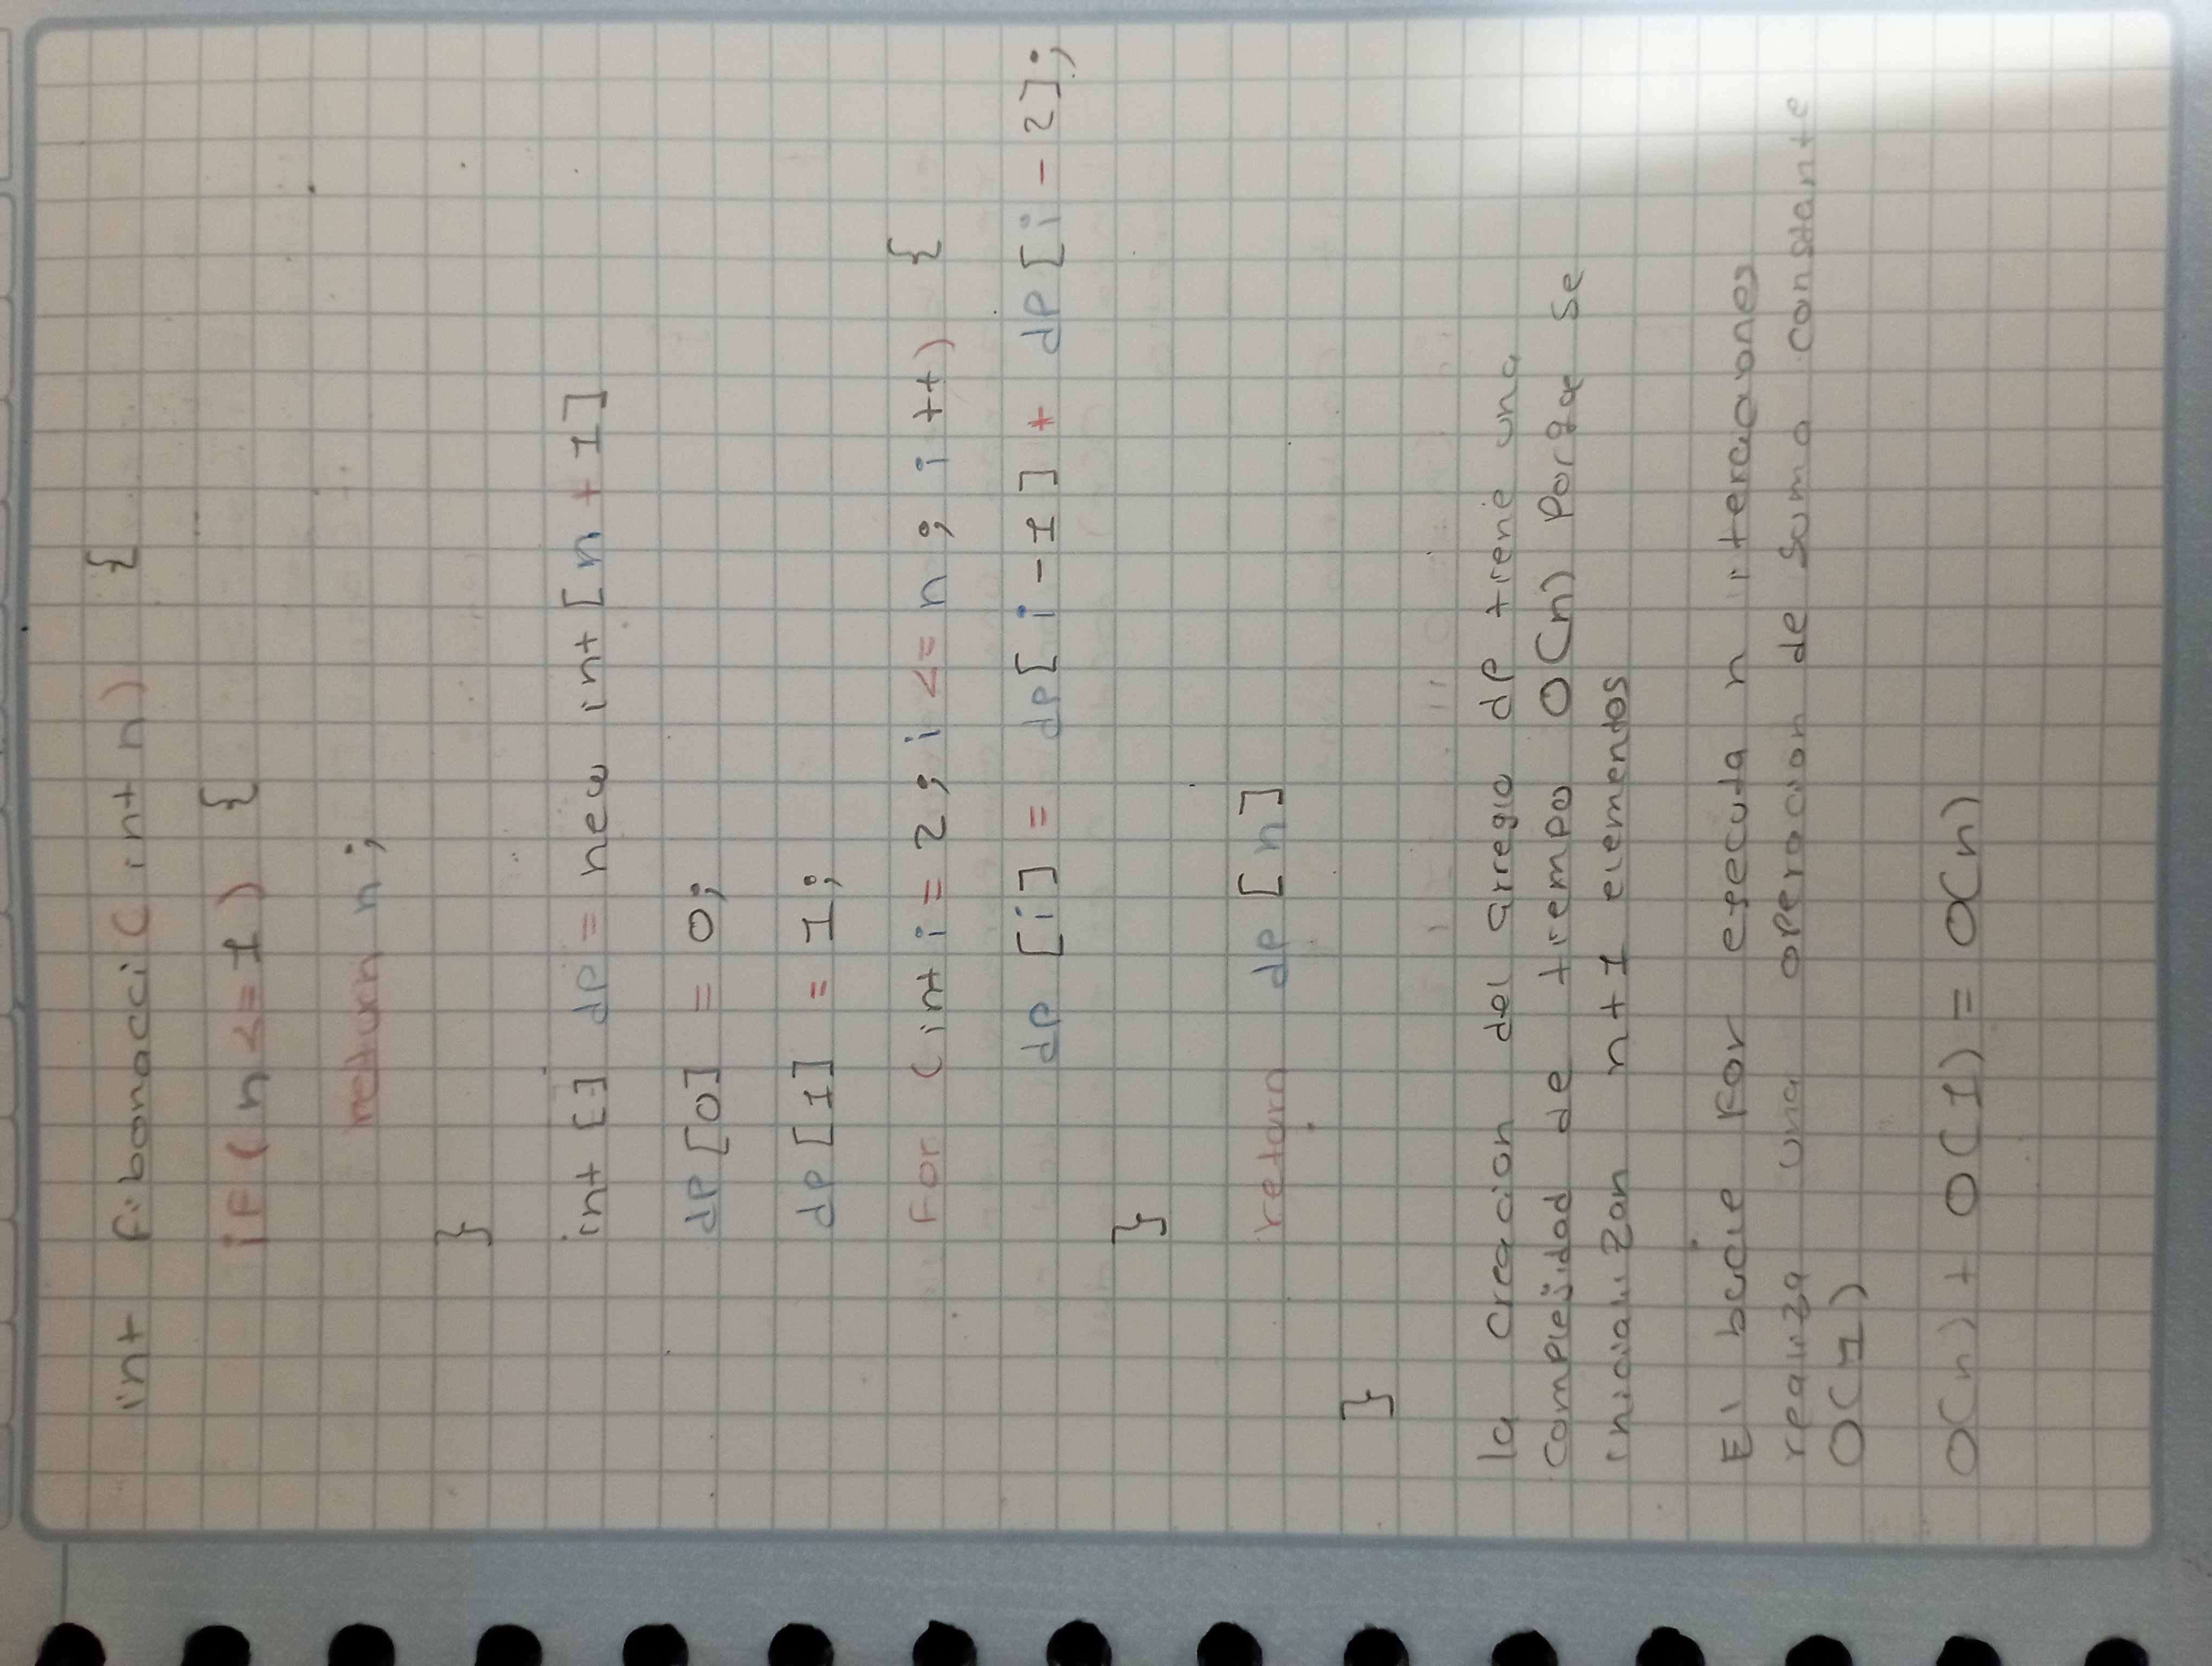
\includegraphics[width=0.5\textwidth]{images/IMG_20230913_023612.jpg}
  \caption{Análisis Escrito Del Algoritmo No. 12}
  \label{fig:nombre_de_tu_imagen}
\end{figure}

La complegidad temporal de este algoritmo es de Big-O O(n) porque calcula los valores de Fibonacci desde 0 hasta "n" en un solo pase a través del bucle.

\subsection{Algoritmo No. 13}

\begin{figure}[H]
  \centering
  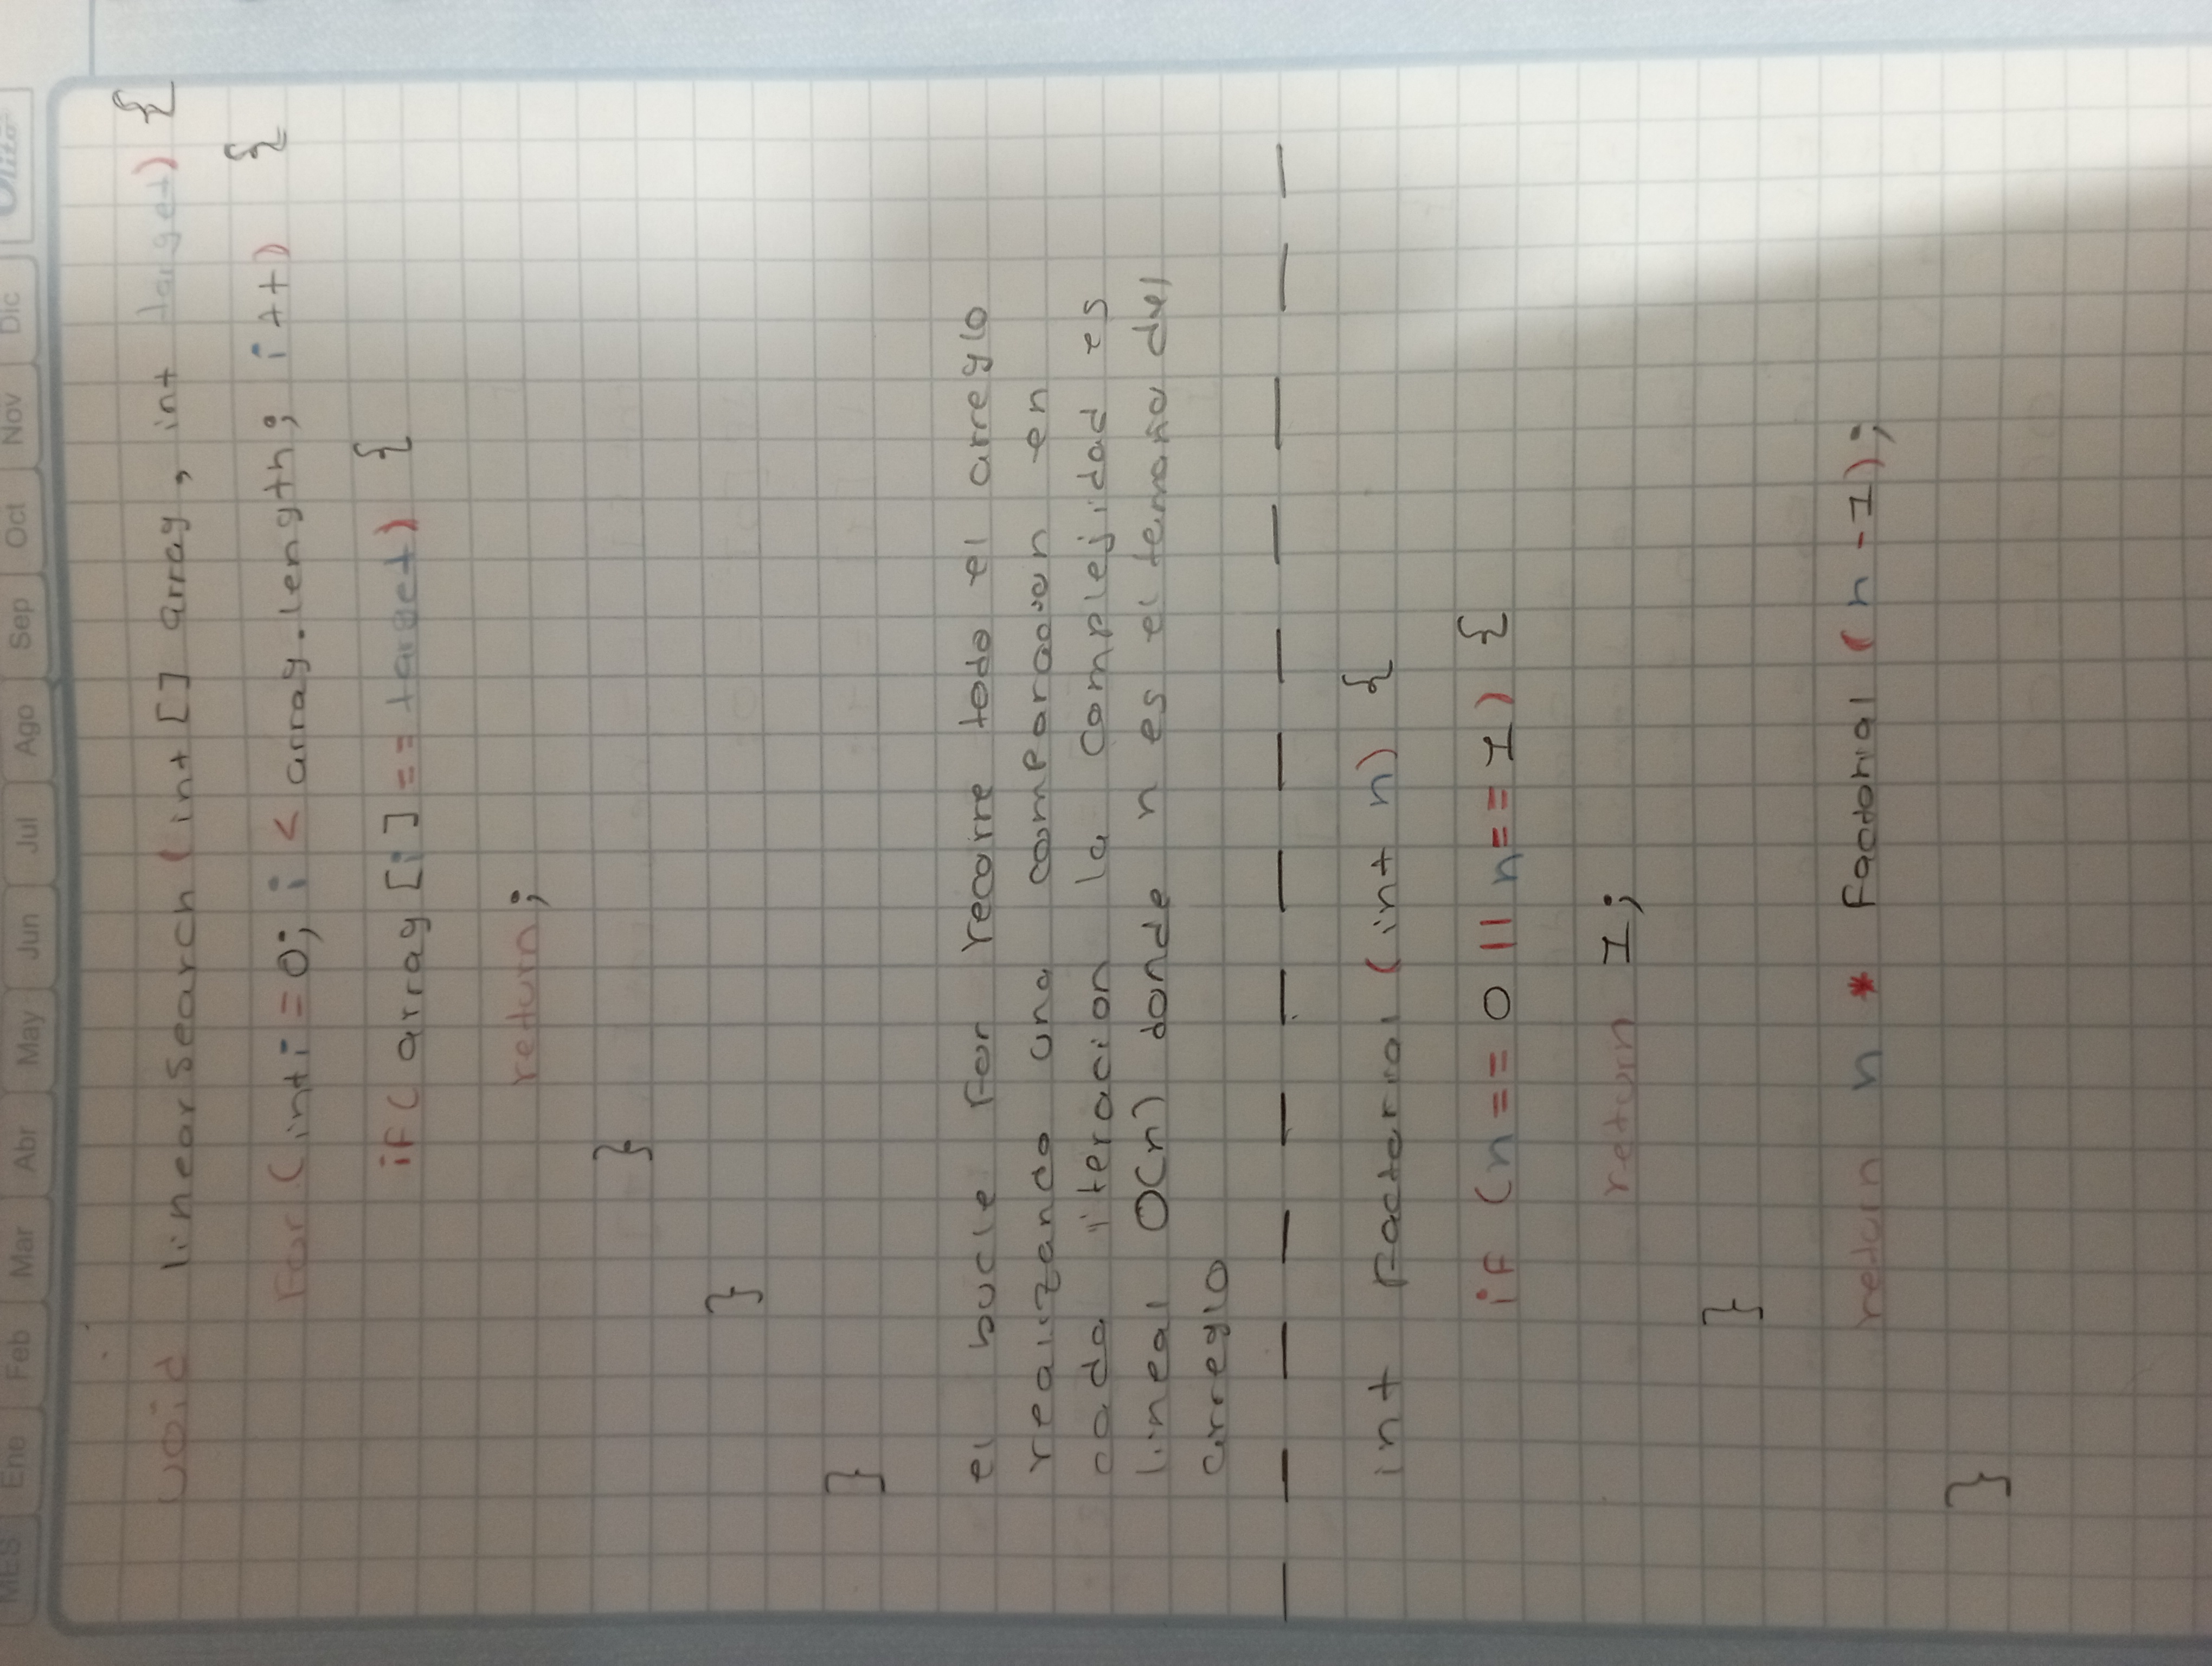
\includegraphics[width=0.5\textwidth]{images/IMG_20230913_023621.jpg}
  \caption{Análisis Escrito Del Algoritmo No. 13}
  \label{fig:nombre_de_tu_imagen}
\end{figure}

La complegidad temporal de este algoritmo es de Big-O O(n), donde "n" es la longitud del array.

\subsection{Algoritmo No. 14}

\begin{figure}[H]
  \centering
  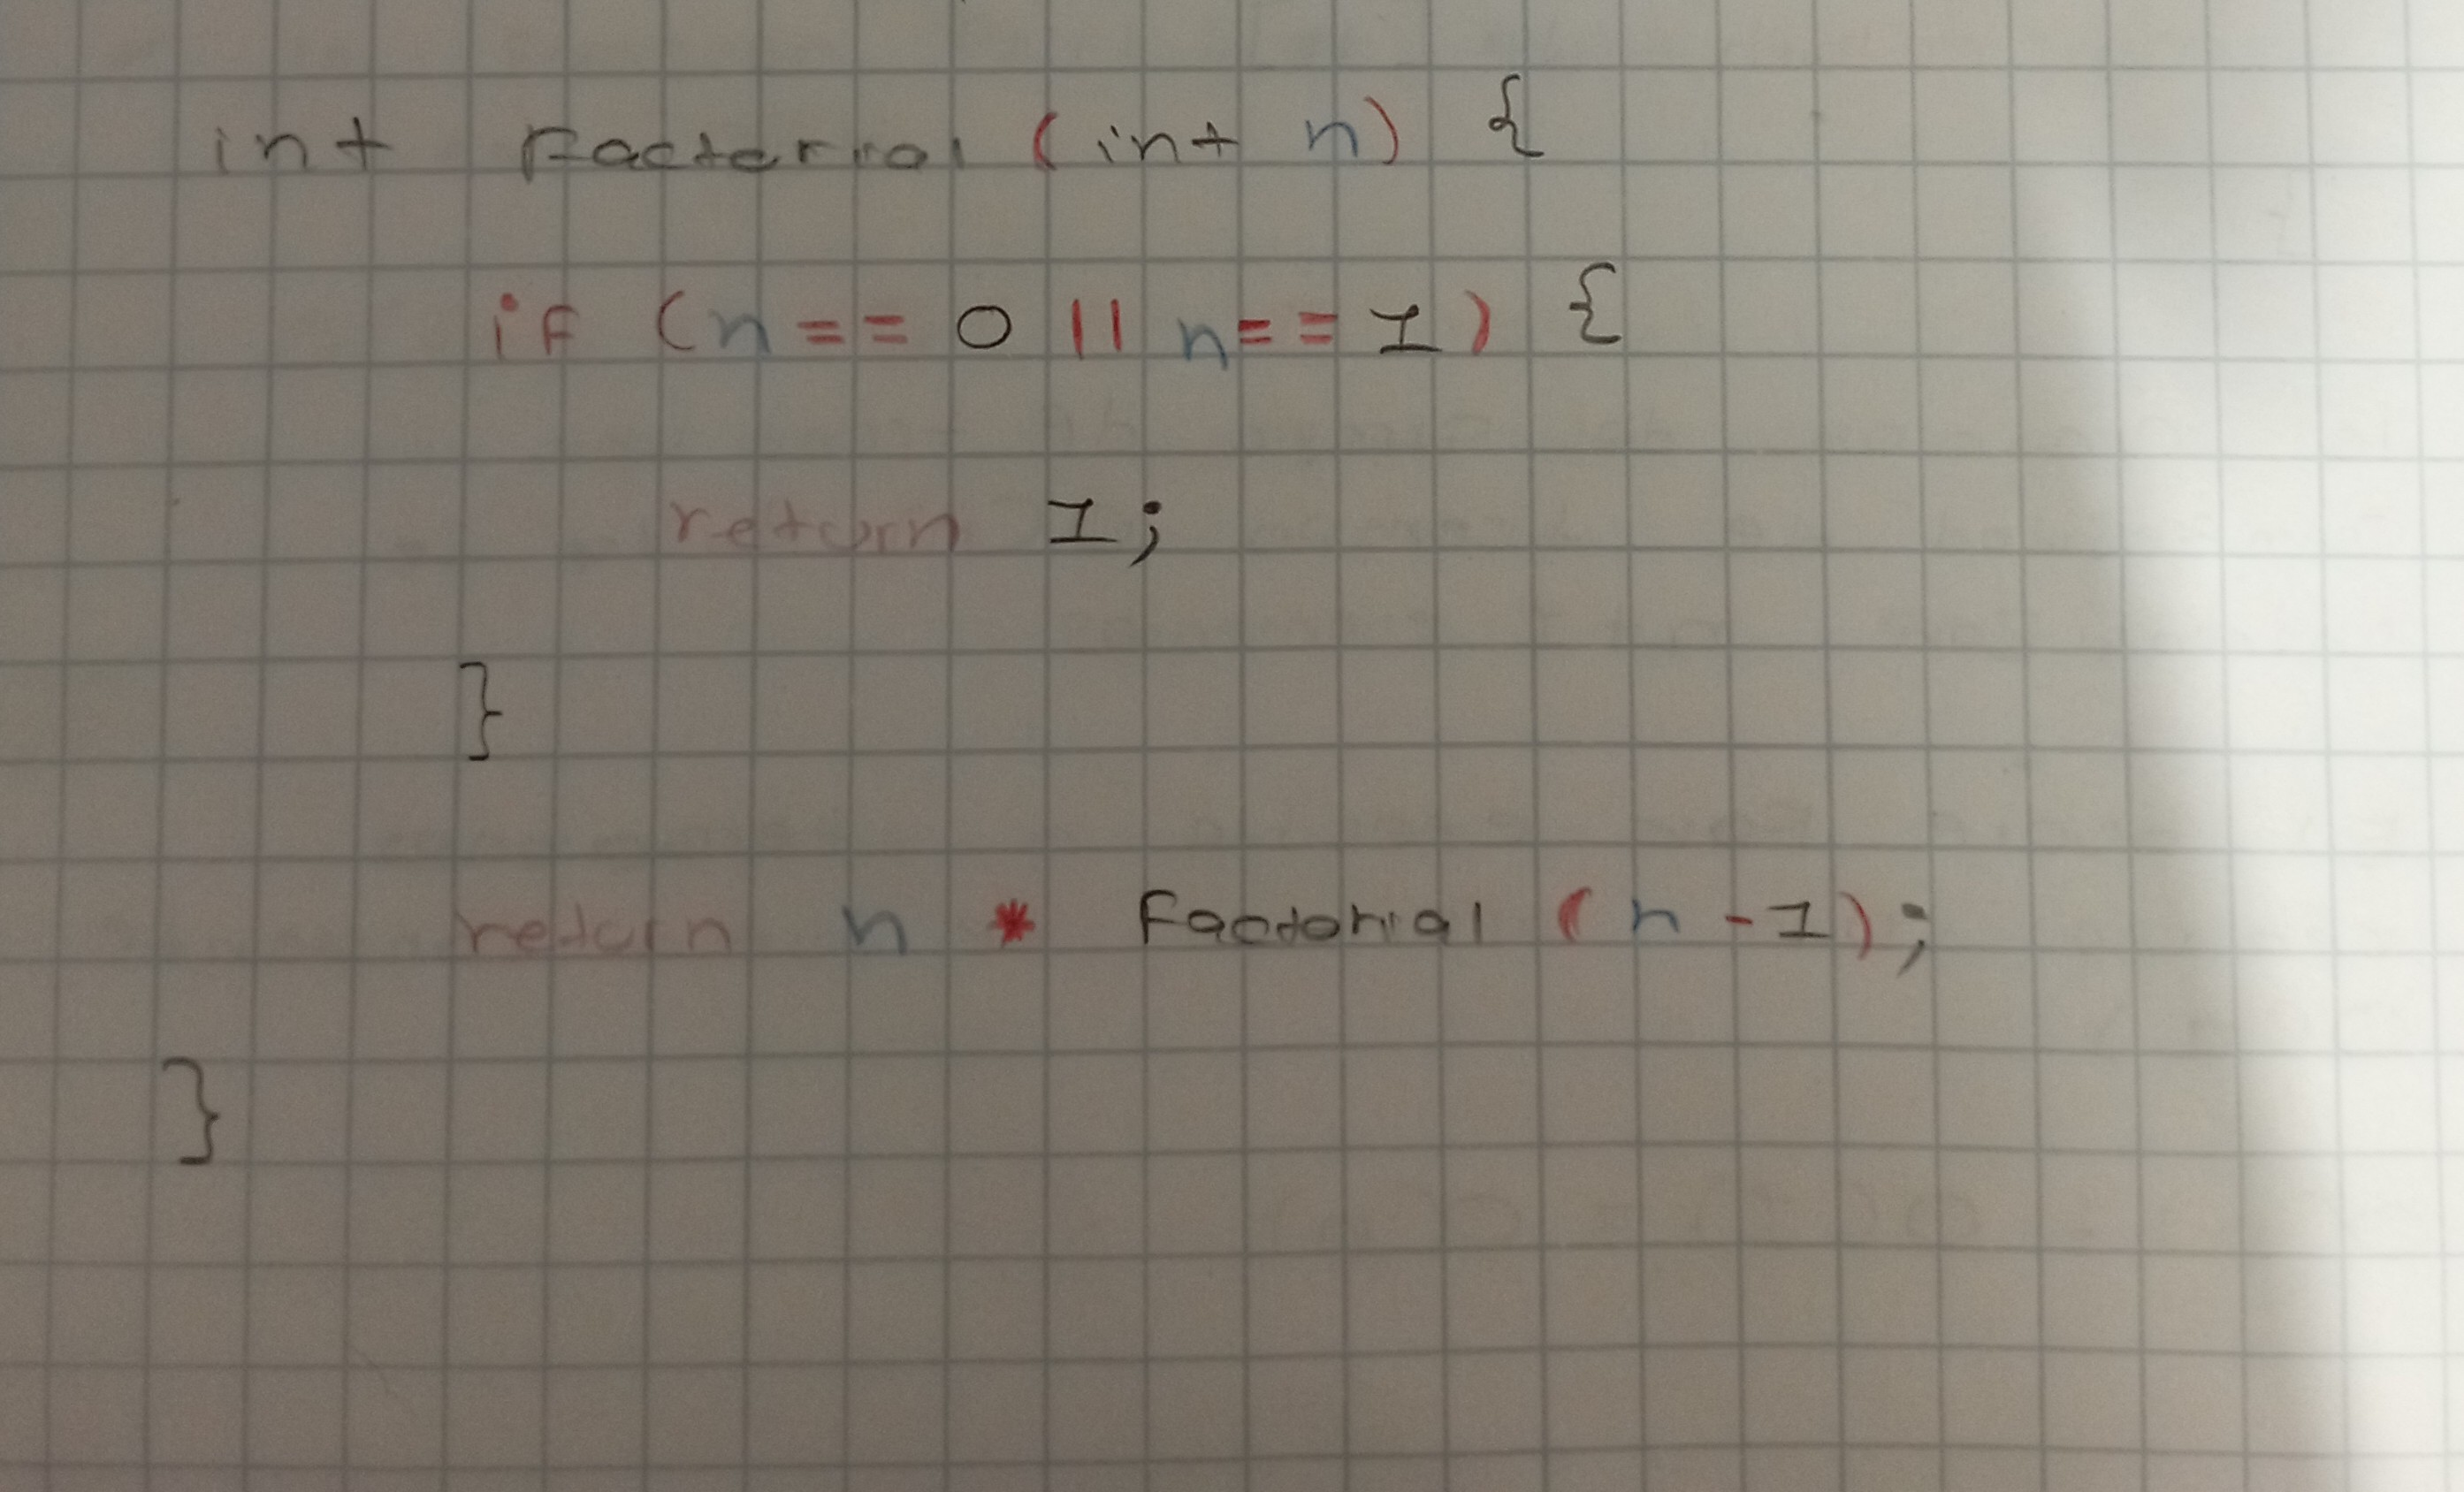
\includegraphics[width=0.5\textwidth]{images/IMG_20230913_023622.jpg}
  \caption{Análisis Escrito Del Algoritmo No. 15 - 1}
  \label{fig:nombre_de_tu_imagen}
\end{figure}

\begin{figure}[H]
  \centering
  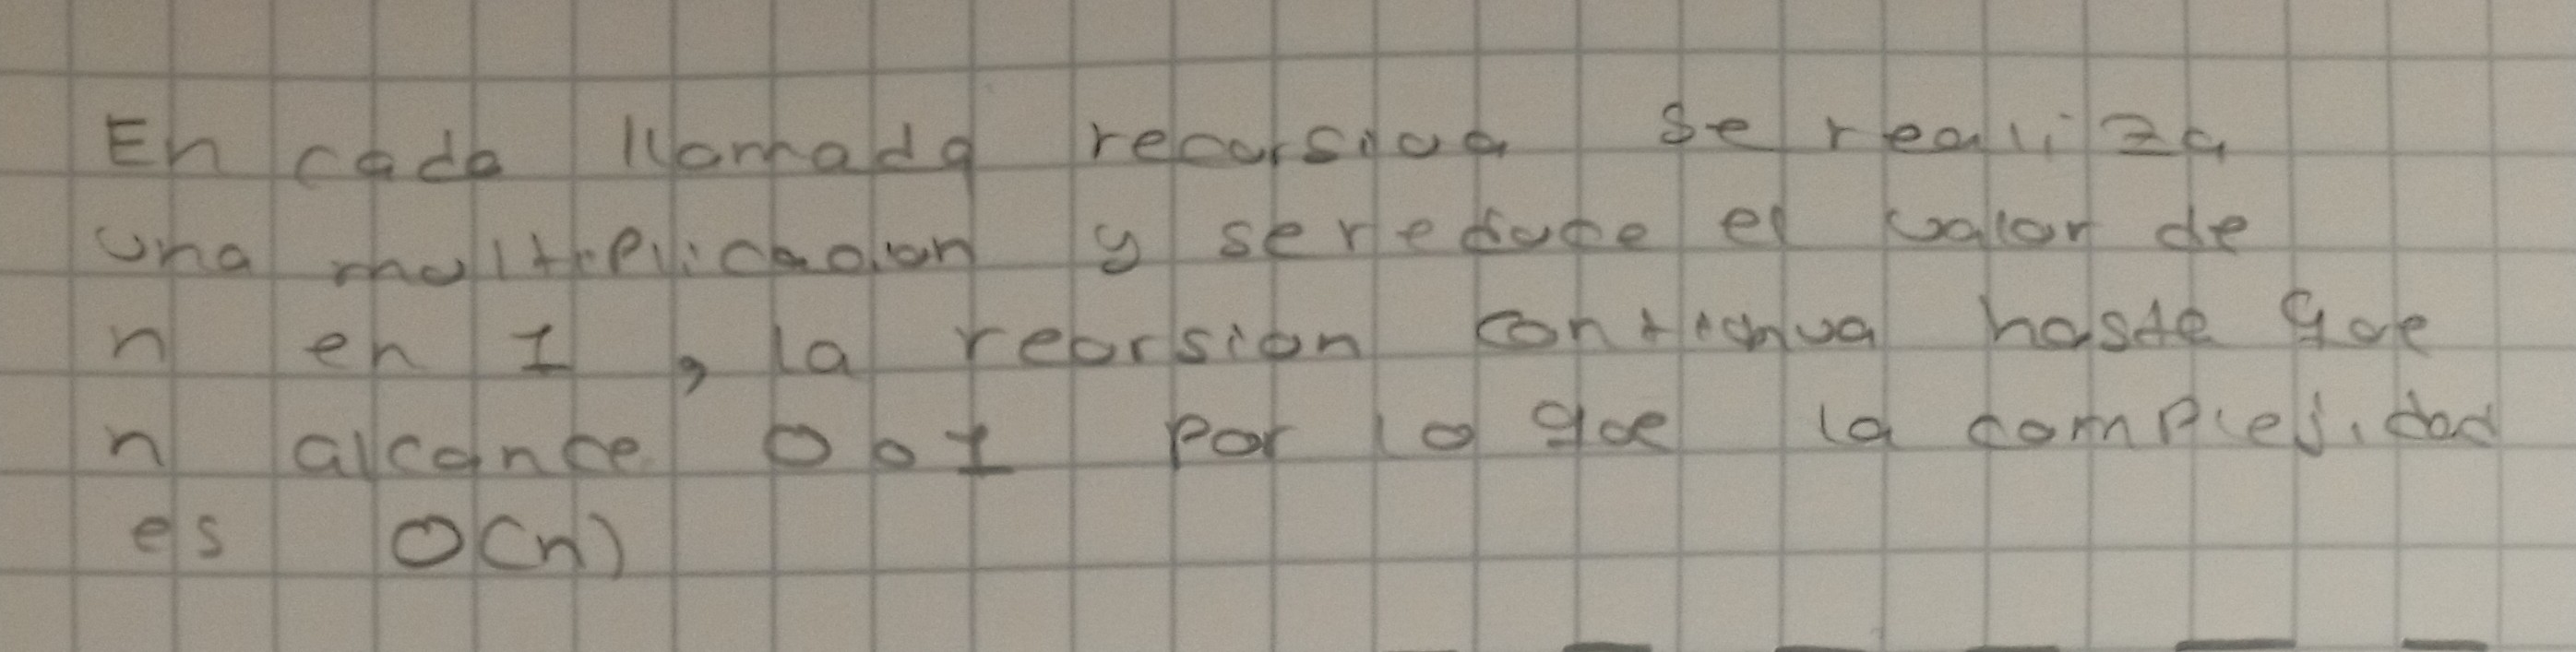
\includegraphics[width=0.5\textwidth]{images/IMG_20230913_023630.jpg}
  \caption{Análisis Escrito Del Algoritmo No. 15 - 2}
  \label{fig:nombre_de_tu_imagen}
\end{figure}

La complegidad temporal de este algoritmo es de Big-O O(n), en términos de llamadas recursivas, ya que se llama a la función factorial n veces.

% Conclusiones
\section{Conclusiones}

Después de realizado el ejercicio de la investigación podemos concluir que los algoritmos dependiendo del planteamiento pueden tener un desempeño óptimo o no en la recursividad de nuestros códigos y que una buena implementación  de los mismos conlleva un buen rendimiento de nuestros servidores y un consumo eficiente de memoria y espacio en disco.

% Bibliografía
\bibliographystyle{IEEEtran}

\bibliography{bibliography}
\vspace{12pt}
\end{document}

